\section{Refinement Verification of SPARCv8}
\label{sec:refine-verification-sparc}

In this section, we present \textit{relational} 
program logic for refinement verification of 
SPARCv8 code. 
% Inspired by the {\it relational} program logic for 
% refinement verification, \eg{\cite{liang13pldi,Xu16cav}}, 
% we extend our program logic for SPARCv8 to support
% refinement verification in this section. 
We first define the high- and low-level program in 
\Sec{\ref{subsec:High-level Pseudo-SPARCv8 Language}} and 
\Sec{\ref{subsec:low-level SPARCv8 Program}} respectively. 
% and their state relation in \Sec{\ref{subsec:state-rel}}. 
The refinement relation is represented in 
\Sec{\ref{subsec:correctness-primitive}}, 
and program logic is shown in \Sec{\ref{subsec:rellogic}}
Finally, logic soundness is shown in 
\Sec{\ref{subsec:semantics and soundness}}.

\subsection{High-level Pseudo-SPARCv8 Language}
\label{subsec:High-level Pseudo-SPARCv8 Language}
% The target program in our work is SPARCv8, which is 
% introduced in \Sec{\ref{sec:modeling}}. So,  
% We choose the SPARCv8 program defined in 
% \Sec{\ref{sec:modeling}} as the {\it low-level} 
% program. And 

The Pseudo-SPARCv8 language contains two part: 
the SPARCv8 code as client code, 
and the set of abstract assembly primitives. 
Here, we require that the execution of client SPARCv8 code 
preserves a restriction between register 
window and stack in memory, shown
as the left side in \Fig{\ref{fig:Abstraction of Register Windows and Memory}}
(\regcwp{} points to the current window and \regwim{} marks 
the invalid window, the details of overlapping 
of adjacent windows are omitted in the figure).
\begin{center}
    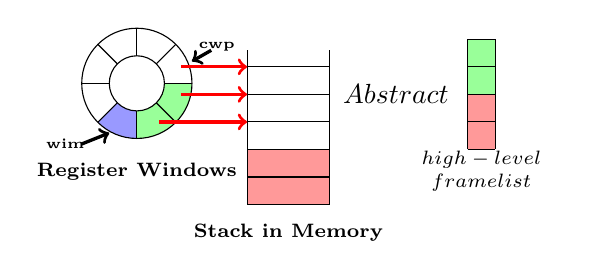
\begin{tikzpicture}[scale=0.7]
    \fill[green!40!white] (0,0) -- (0,-1cm) arc (-90:0:1cm) -- (0,0);
    \fill[blue!40!white] (0,0) -- (0,-1cm) arc (-90:-135:1cm) -- (0,0);
    % \fill[yellow!80!white] (0,0) -- (0,-1cm) arc (-90:-135:1cm) -- (0,0);
    % \fill[blue!40!white] (0,0) -- (-1,0cm) arc (-180:-135:1cm) -- (0,0);
    \draw (0, 0) -- (90:1cm);
    \draw (0, 0) -- (45:1cm);
    \draw (0, 0) -- (0:1cm);
    \draw (0, 0) -- (-45:1cm);
    \draw (0, 0) -- (-90:1cm);
    \draw (0, 0) -- (-135:1cm);
    \draw (0, 0) -- (-180:1cm);
    \draw (0, 0) -- (135:1cm);
    \fill[white] (0, 0) circle (0.5cm);
    \draw (0, 0) circle (1cm);
    \draw (0, 0) circle (0.5cm);
    % \draw[very thick, blue] (0, -0.3) -- (0, -1.2);
    % \draw[very thick, blue] (0, -0.32) -- (0.1, -0.32);
    % \draw[very thick, blue] (0, -1.18) -- (0.1, -1.18);
    \node(wim) at (-1.3, -1.1) {\tiny \bf wim};
    \draw[->, very thick] (-1, -1.1) -- (-0.5, -0.9);

    % \node(wim) at (-1.7, -0.7) {\tiny \bf wim};
    % \draw[->, very thick] (-1.5, -0.6) -- (-1, -0.4);
    

    \node(cwp) at (1.45, 0.67) {\tiny \bf cwp};
    \draw[->, very thick] (1.35, 0.6) -- (1, 0.4);

    \node(regwin) at (0, -1.6) {\scriptsize \bf Register Windows};

    %%%%%%%%%%%%%%%%%%%%%%%%%%%%%%%%%%%%%%%%%%%%%%%%%%%%%%

    \fill[red!40!white] (2, -1.2) rectangle (3.5, -1.7);
    \fill[red!40!white] (2, -1.7) rectangle (3.5, -2.2);

    \draw[-] (2, 0.6) -- (2, -2.2);
    \draw[-] (3.5, 0.6) -- (3.5, -2.2);
    
    \draw[-] (2, 0.3) -- (3.5, 0.3);
    \draw[-] (2, -0.2) -- (3.5, -0.2);
    \draw[-] (2, -0.7) -- (3.5, -0.7);
    \draw[-] (2, -1.2) -- (3.5, -1.2);
    \draw[-] (2, -1.7) -- (3.5, -1.7);
    \draw[-] (2, -2.2) -- (3.5, -2.2);

    \node(stkfm) at (2.75, -2.7) {\scriptsize \bf Stack in Memory};

    %%%%%%%%%%%%%%%%%%%%%%%%%%%%%%%%%%%%%%%%%%%%%%%%%%%%%%%

    \draw[->, very thick, red] (0.8, 0.3) -- (2, 0.3);
    \draw[->, very thick, red] (0.8, -0.2) -- (2, -0.2);
    \draw[->, very thick, red] (0.4, -0.7) -- (2, -0.7);

    %%%%%%%%%%%%%%%%%%%%%%%%%%%%%%%%%%%%%%%%%%%%%%%%%%%%%%

    \node(abstract) at (4.7, -0.2) {$\xLongrightarrow{\text{Abstract}}$};

    %%%%%%%%%%%%%%%%%%%%%%%%%%%%%%%%%%%%%%%%%%%%%%%%%%%%%%

    \fill[green!40!white] (6, 0.8) rectangle (6.5, 0.3);
    \fill[green!40!white] (6, 0.3) rectangle (6.5, -0.2);
    \fill[red!40!white] (6, -0.2) rectangle (6.5, -0.7);
    \fill[red!40!white] (6, -0.7) rectangle (6.5, -1.2);

    \draw[-] (6, 0.8) -- (6, -1.2);
    \draw[-] (6.5, 0.8) -- (6.5, -1.2);

    \draw[-] (6, 0.8) -- (6.5, 0.8);
    \draw[-] (6, 0.3) -- (6.5, 0.3);
    \draw[-] (6, -0.2) -- (6.5, -0.2);
    \draw[-] (6, -0.7) -- (6.5, -0.7);
    \draw[-] (6, -1.2) -- (6.5, -1.2);

    \node(hfrmlist) at (6.25, -1.6) 
        {
            \scriptsize \bf
            $
            \begin{array}{c}
                \text{high-level} \\
                \text{framelist}
            \end{array}
            $
        };
\end{tikzpicture} 
    \vspace*{-0.5em}
    \figurecaption{Abstraction of context management}
    \label{fig:Abstraction of Register Windows and Memory}
    \vspace{-0.5em}
\end{center}
During the SPARCv8 program's execution, 
part of previous procedures' contexts 
(the green part in the left side of the 
\Fig{\ref{fig:Abstraction of Register Windows and Memory}}) 
are saving in register window, the others 
(the pink part in the left side of the 
\Fig{\ref{fig:Abstraction of Register Windows and Memory}})
are stored in stack in memory, 
% (shown as the red arrow in 
% \Fig{\ref{fig:Abstraction of Register Windows and Memory}}), 
because the number of windows is limited. 
The restriction is that the stack pointer 
(\spreg{}) of each procedure, 
including the current one and the previous one, 
whose contexts are saved in register 
window currently, should point to the top of its stack frame 
(shown as the red arrow in 
\Fig{\ref{fig:Abstraction of Register Windows and Memory}}),
so that the contexts 
in these windows can be stored correctly 
in memory when needed. For instance,  
the context switch routine will check 
whether the previous window is valid 
(in clockwise direction in 
\Fig{\ref{fig:Abstraction of Register Windows and Memory}}), 
and use instruction $\crestore{}$ to set it as the 
current one and save its contents into stack 
(in memory) until the previous one is invalid 
(marked in blue in \Fig{\ref{fig:Abstraction of Register Windows and Memory}}). 
We require the execution of client code 
preserving such restriction. Otherwise, some SPARCv8 
functions like context switch routine whose 
implementations will store the contexts saved in 
register window into stack in memory cannot be 
verified if it's unclear where to save the 
contents of some windows. 
% We require the execution of client code 
% preserving this relation so that the relation 
% holds when calling context switch routine. 
% \footnote{The requirement for client code
% preserving such relation will not restrict the 
% application of our work, because such relation
% is also mentioned as a SPARCv8 programming 
% convention in The SPARC Architecture Manual(version 8)~\cite{sparc},
% which says that "It is essential 
% that \spreg{} always contains the correct value, 
% so that when (and if) a register window overflow/underflow trap occurs, 
% the register window can be correctly stored to or reloaded from memory "}.
% Otherwise, the correctness of context switch 
% routine can't be proved if we are unclear where 
% to save the contents of some windows. 
We do the following when defining 
Pseudo-SPARCv8 program to make the execution 
of client code preserves such restriction:  
\begin{itemize}
    \item
    In order to ensure that 
    the stack pointer (\spreg{}) always 
    points to the top of its stack frame, we require that   
    each instruction, like \cadd{} and \ld{}, whose 
    execution will not rotate register window, 
    is not allowed to update the value of \spreg{}; 
    and as for the \csave{} and \crestore{}, 
    % whose executions 
    % will rotate register window, 
    we require them 
    to be used in specific forms. 
    We introduce ``$\Psave \ \word$" as a macro of 
    ``$\csave{} \ \spreg, -\word, \spreg$", 
    whose execution makes sure that a new \spreg{} 
    will be generated for the next window
    and point to the stack frame size $w$ allocated newly. 
    We also introduce ``$\Prestore$" 
    as a macro of ``$\crestore{} \ \greg{0}, \greg{0}, \greg{0}$"
    \footnote{In SPARCv8, $\greg{0}$ is always equal to 0, 
    and usually used as parameters when instructions do not 
    require specific parameters.},  
    whose execution just restores the previous window 
    and doesn't modify the value of any register 
    in the previous window restored. 
    The original \csave{} and \crestore{} instructions 
    have \textit{no} semantics in high-level client code.   
    
    % The \csave{} and \crestore{} instructions that operate  
    % register window can't be used arbitrarily. 
    % When we use \csave{} to rotate to next window
    % (counterclockwise direction in \Fig{\ref{fig:Abstraction of Register Windows and Memory}}),  
    % a new stack pointer \spreg{} should 
    % be generated to point to the stack frame 
    % in memory allocated newly. 
    % And when we use \crestore{} to rotate to previous window 
    % (in clockwise direction in \Fig{\ref{fig:Abstraction of Register Windows and Memory}}), 
    % its execution shouldn't modify x
    % the value of \spreg{} in the previous window.
    % % So as to preserve the requirement that each 
    % % stack pointer (\spreg) points 
    % % to its corresponding stack frame
    % % during the execution of client code,  
    % % the execution of \csave{} should generate a new 
    % % \spreg{} pointing to the stack frame in 
    % % memory allocated newly, and the execution of 
    % % \crestore{} shouldn't modify the value of 
    % % \spreg{} in the window restored.  
    % So, we introduce ``$\Psave \ \word$" as a macro of 
    % ``$\csave{} \ \spreg, -\word, \spreg$", 
    % whose execution makes sure that a new \spreg{} 
    % will be generated and point to the stack frame 
    % size $w$ allocated newly. 
    % We also introduce ``$\Prestore$" 
    % as a macro of ``$\crestore{} \ \greg{0}, \greg{0}, \greg{0}$"
    % \footnote{In SPARCv8, $\greg{0}$ is always equal to 0, 
    % and usually used as parameters when instructions do not 
    % require specific parameters.},  
    % whose execution just restores the previous window 
    % and doesn't modify any register value. 
    % The original \csave{} and \crestore{} instructions 
    % have \textit{no} semantics in high-level client code. 

    \item 
    % The special registers can't be modified arbitrarily.
    The special registers in SPARCv8 usually act specific 
    roles and modifying them should be carefully, 
    \begin{center}
        \vspace*{-0.5em}
        \begin{tikzpicture}[scale=0.75]
    \pgfdeclarepatternformonly{my crosshatch dots}{\pgfqpoint{-1pt}{-1pt}}{\pgfqpoint{2.5pt}{2.5pt}}{\pgfqpoint{3pt}{3pt}}
    {
        \pgfpathcircle{\pgfqpoint{0pt}{0pt}}{.4pt}
        \pgfpathcircle{\pgfqpoint{1.5pt}{1.5pt}}{.4pt}
        \pgfusepath{fill}
    }

    \fill[gray!20] (0,0) -- (0,-1cm) arc (-90:0:1cm) -- (0,0);
    \fill[pattern=my crosshatch dots] (0,0) -- (0,-1cm) arc (-90:-135:1cm) -- (0,0);
    \fill[pattern=north east lines] (0,0) -- (-1,0cm) arc (-180:-135:1cm) -- (0,0);
    \draw (0, 0) -- (90:1cm);
    \draw (0, 0) -- (45:1cm);
    \draw (0, 0) -- (0:1cm);
    \draw (0, 0) -- (-45:1cm);
    \draw (0, 0) -- (-90:1cm);
    \draw (0, 0) -- (-135:1cm);
    \draw (0, 0) -- (-180:1cm);
    \draw (0, 0) -- (135:1cm);
    \fill[white] (0, 0) circle (0.5cm);
    \draw (0, 0) circle (1cm);
    \draw (0, 0) circle (0.5cm);

    \node(wim) at (-1.7, -0.7) {\tiny \bf wim};
    \draw[->, line width=0.5pt] (-1.5, -0.6) -- (-1, -0.4);
    

    \node(cwp) at (1.45, 0.67) {\tiny \bf cwp};
    \draw[->, line width=0.5pt] (1.35, 0.6) -- (1, 0.4);

    \node(regwin) at (0, -1.6) {\scriptsize Register Windows};

    %%%%%%%%%%%%%%%%%%%%%%%%%%%%%%%%%%%%%%%%%%%%%%%%%%%%%%

    \fill[black!50] (2, -1.2) rectangle (3.3, -1.7);
    \fill[black!50] (2, -1.7) rectangle (3.3, -2.2);

    \draw[-] (2, 0.6) -- (2, -2.2);
    \draw[-] (3.3, 0.6) -- (3.3, -2.2);
    
    \draw[-] (2, 0.3) -- (3.3, 0.3);
    \draw[-] (2, -0.2) -- (3.3, -0.2);
    \draw[-] (2, -0.7) -- (3.3, -0.7);
    \draw[-] (2, -1.2) -- (3.3, -1.2);
    \draw[-] (2, -1.7) -- (3.3, -1.7);
    \draw[-] (2, -2.2) -- (3.3, -2.2);

    \node(stkfm) at (2.75, -2.7) {\scriptsize Stack in Memory};

    %%%%%%%%%%%%%%%%%%%%%%%%%%%%%%%%%%%%%%%%%%%%%%%%%%%%%%%

    \draw[->, line width=0.8pt] (0.8, 0.3) -- (2, 0.3);
    \draw[->, line width=0.8pt] (0.8, -0.2) -- (2, -0.2);
    \draw[->, line width=0.8pt] (0.4, -0.7) -- (2, -0.7);

    %%%%%%%%%%%%%%%%%%%%%%%%%%%%%%%%%%%%%%%%%%%%%%%%%%%%%%

    % \node(abstract) at (4.7, -0.2) {$\xLongrightarrow{\text{Abstract}}$};

    %%%%%%%%%%%%%%%%%%%%%%%%%%%%%%%%%%%%%%%%%%%%%%%%%%%%%%
\end{tikzpicture} 
        \figurecaption{Problem of modifying 
        \regwim{} arbitrary}
        \vspace*{-0.5em}
        \label{fig:problem of modifying wim arbitrary}
    \end{center}
    for example, \regwim{} marks which window is 
    invalid. If we change its value shown in 
    \Fig{\ref{fig:Abstraction of Register Windows and Memory}}, 
    to mark another window invalid, as shown in 
    \Fig{\ref{fig:problem of modifying wim arbitrary}}, 
    and call context switch routine, which will  
    save the contents of previous windows into memory
    until the invalid one, at this moment. 
    There will be a problem that we don't know 
    where to save the contents of window that 
    is marked invalid originally 
    (window in yellow in \Fig{\ref{fig:problem of modifying wim arbitrary}}). 
    % Supposing the register window and  
    So, we don't allow client code 
    to modify special registers and do \textit{not} 
    give semantics to \cwr{} instruction in high-level 
    client code. Modifying them is hidden in the 
    implementation of the abstract assembly primitives
    in low-level. 
    And the delay buffer can be omitted in high-level
    program state. 
    % omit them 
    % in the Pseudo-SPARCv8 program state. Operating them 
    % is hidden in the implementation of the 
    % abstract assembly primitives. 
    % We also do \textit{not} give semantics to 
    % \cwr{} and \rd{} instructions in high-level 
    % client code. 
    \item 
    As shown in \Fig{\ref{fig:Abstraction of Register Windows and Memory}}, 
    we find that we can abstract the register window 
    and the memory in stack for storing contexts 
    as a list (defined as 
    HFrmList formally in \Fig{\ref{fig:machine-state-concur-pseudo-sparc}}).  
    After this abstraction, We don't need to care about 
    whether the contexts are saved in register window or 
    memory, and don't need to describe the contents of windows unused 
    (the windows in white color in 
    \Fig{\ref{fig:Abstraction of Register Windows and Memory}}, 
    but excluding the current one pointed by \regcwp{}) 
    in the Pseudo-SPARCv8 level. 
    The \regcwp{} register is no longer needed in 
    Pseudo-SPARCv8 program because the register window 
    is abstracted away. 
    The low-level program in our work doesn't use this 
    abstraction, because the low-level program 
    should be realistically modelled, 
    and the implementations of some primitives 
    need to know the existance of register window,  
    for instance, the context switch routine 
    needs to save the contents 
    of the register window into stack (in memory).
\end{itemize}

\begin{figure*}[!t]
    \centering
    \vspace{-2em}
    \small
    \[
        \begin{array}{rcclcrccl}
            \TYPE{(HCode)} & \ \HMd \ & \define & (\code, \hprimset) & & 
            \qquad\,
            \TYPE{(CodeHeap)} & \ \code \ & \in & \TYPE{Word} \rightharpoonup \TYPE{Comm} 
            \\
            \\[-8pt]
            \TYPE{(PrimSet)} & \hprimset & \define & 
            \multicolumn{6}{l}
                {
                    \{ \lab{1} \rightsquigarrow \hprim_1, \dots, \lab{n} \rightsquigarrow \hprim_n \}
                    \qquad\quad
                    \TYPE{(Prim)} \ \ \hprim \ \in \ 
                    \TYPE{List} \ \TYPE{Val} \rightarrow \TYPE{HState} \rightarrow 
                    \TYPE{HState} \rightarrow \TYPE{Prop}            
                }  \\
            \\
            % \TYPE{(Prim)} & \hprim & \in & 
            % \multicolumn{6}{l}
            % {
            %     \TYPE{List} \ \TYPE{Val} \rightarrow \TYPE{HState} \rightarrow 
            %     \TYPE{HState} \rightarrow \TYPE{Prop}
            % } \\
            % \TYPE{(OpExp)} & \oexp & \define & \reg{} \sepline \val & & 
            % \TYPE{(AddrExp)} & \aexp & \define & \oexp \sepline \reg{} + \oexp \\
            \TYPE{(Comm)} & \comm & \define & 
            \multicolumn{6}{l}
            {
                \simplins{} \sepline \call{} \ \lab{} 
                \sepline \jmp{} \ \aexp \sepline \retl \sepline \be{} \ \lab{}
            }  
            \\
            \\[-8pt]
            \TYPE{(SimpIns)} & \simplins{} & \define & 
            \multicolumn{6}{l}
            {
                % \csave{} \ \reg{s} \ \oexp \ \reg{d} \sepline 
                % \crestore{} \ \reg{s} \ \oexp \ \reg{d} \sepline
                \Psave \ \word \sepline \Prestore  \sepline \cprint \ \reg{} \sepline 
                \ld{} \ \aexp \ \reg{d} \sepline 
                \st{} \ \reg{s} \ \aexp \sepline \cadd{} \ \reg{s} \ \oexp \ \reg{d}
                \sepline
                \rd \ \sr \ \reg{d} \sepline \cwr \ \reg{s} \ \oexp \ \sr 
                % \sepline \dots
            } 
            \\
            & & \quad | & 
            \multicolumn{6}{l}
            {
                \csave{} \ \reg{s} \ \oexp \ \reg{d} \sepline 
                \crestore{} \ \reg{s} \ \oexp \ \reg{d} \sepline
                \dots
            } 
            \\
            \\[-8pt]
            \TYPE{(HMsg)} & \hmsg & \define & \empmsg \sepline \outEvt{\val} \sepline 
            \callEvt{\lab{}, \args{\val}} 
        \end{array}
    \]
    \vspace{-1em}
    \caption{Syntax of Pseudo-SPARCv8 Code}
    \label{fig:syntax-of-concur-pseudo-sparc}
    \vspace{-1em}
\end{figure*}
\begin{figure*}[!t]
    \centering
    \small
    \[
        \begin{array}{rcclrcclrccl}
            \TYPE{(HProg)} & \ \HProg \ & \define & 
            (\HMd, \hpstate) &
            \TYPE{(HState)} & \hpstate & \define & 
            \multicolumn{3}{l}
            {
                (\thrdpool, \thrdid, \hthrdlocalst, \Mem)
            }
            % \multicolumn{7}{l}
            % {
            %     \TYPE{(HState)} \ \ \hpstate \ \ 
            %     \define \ \ 
            %     (\thrdpool, \thrdid, \hthrdlocalst, \Mem)
            % } 
            \\
            \\[-8pt]
            \TYPE{(ThrdPool)} & \thrdpool & \define & 
            \{ \thrdid \rightsquigarrow \hthrdlocalst \}^{*}
            & \ \ 
            \TYPE{(ThrdLcSt)} & \ \hthrdlocalst \ & \define & 
            (\hRstate, \pc, \npc) 
            & \qquad
            \TYPE{(Tid)} & \thrdid & \in & \Ztype \\
            \\
            \TYPE{(HRstate)} & \hRstate & \define & 
            (\hRfile, \hWstk) \\
            \\[-8pt]
            \TYPE{(HRegFile)} & \hRfile & \in & 
            \TYPE{HRegName} \rightarrow \TYPE{Val} 
            & \quad
            \TYPE{(HRegName)} & \hrn & \define & 
            \multicolumn{5}{l}
            {
                \reg{0} \sepline \dots \sepline \reg{31} \sepline 
                \regn \sepline \regz \sepline \regc \sepline \regv 
            } \\
            \\[-8pt]
            \TYPE{(HFrmList)} & \hWstk & \define & 
            \nil \sepline (\fm_1, \fm_2) \stCons \hWstk
            & \qquad
            \TYPE{(HFrame)} & \fm & \define & 
            [\val_0, \dots, \val_7]
        \end{array}
        % \begin{array}{rcclcrccl}
        %     \TYPE{(HProg)} & \ \HProg \ & \define & 
        %     (\HMd, \hpstate, \pc, \npc) 
        %     & \ \ &
        %     \TYPE{(HState)} & \hpstate & \define & (\thrdpool, \thrdid, \hthrdlocalst, \Mem) \\
        %     \TYPE{(ThrdPool)} & \ \thrdpool \ & \define & 
        %     \{ \thrdid \rightsquigarrow \hthrdlocalst \}^{*} & & 
        %     \TYPE{(ThrdLcSt)} & \hthrdlocalst & \define & (\hRstate, \pc, \npc) \\ 
        %     \TYPE{(HRstate)} & \hRstate & \define & (\hRfile, \block, \hWstk) & & 
        %     \TYPE{(ProgCount)} & 
        %     \multicolumn{3}{l}
        %     {
        %         \, \pc, \npc \ \in \ \TYPE{Word}
        %     }
        %     \\
        %     \TYPE{(Tid)} & \thrdid & \in & \Ztype & & 
        %     \TYPE{(HRegFile)} & \hRfile & \in & 
        %         \TYPE{HRegName} \rightharpoonup \TYPE{Val} \\ 
        %     \TYPE{(HRegName)} & \hrn & \define & 
        %     \multicolumn{6}{l}
        %     {
        %         \reg{0} \sepline \dots \sepline \reg{31} \sepline 
        %         \regn \sepline \regz \sepline \regc \sepline \regv
        %     } \\
        %     \TYPE{(HFrmList)} & \hWstk & \define & 
        %     \nil \sepline (\block, \fm_1, \fm_2) \stCons \hWstk & & 
        %     \TYPE{(HFrame)} & \fm & \define & [\val_0, \dots, \val_7]  
        % \end{array}
    \]
    \vspace{-1em}
    \caption{Machine States for Pseudo-SPARCv8 Code}
    \label{fig:machine-state-concur-pseudo-sparc}
    \vspace{-0.5em}
\end{figure*}

We define the syntax of the high-level Pseudo-SPARCv8 language 
in \Fig{\ref{fig:syntax-of-concur-pseudo-sparc}}. 
The code $\HMd$ has two parts : 
the code heap $\code$ 
and a set of abstract primitives $\hprimset$, 
which is a partial mapping from labels to 
abstract assembly primitive. The code heap $\code$ in $\HMd$ 
acts as the client code to 
call abstract assembly primitive. 
The abstract assembly primitive $\hprim$ 
is defined as a relation that takes a list of values 
as arguments and maps a high-level program state 
(defined in \Fig{\ref{fig:machine-state-concur-pseudo-sparc}}) 
to another. 
% The definition of command and simple instruction are similar with 
% the ones defined in \Fig{\ref{fig:Machine States and Language for SPARC Code}}, 
% except that we add two pseudo instructions $\Psave \ \word$ and $\Prestore$ 
% in simple instruction.
% Comparing the simple instruction with the one shown in 
% \Fig{\ref{fig:Machine States and Language for SPARC Code}}, 
% we add three pseudo instructions. 
We add three pseudo instruction in simple instruction. 
The $\Psave \ \word$ 
and $\Prestore$ restrict the \csave{} and \crestore{}
instructions can only be used in specific form as 
mentioned before.  
% saves the contents of the current window and 
% allocate a new stack frame of size $\word$ bytes for new procedure. 
% The $\Prestore$ is responsible for 
% freeing the current stack frame and 
% restore the contents of the previous window. 
% we add two pseudo instructions $\Psave \ \word$ and $\Prestore$ 
% in simple instruction. 
% In the introduction of the example shown in 
% \Fig{\ref{fig:An Example for SPARC Code}}, we say that the instruction 
% ``$\csave{} \ \spreg, -64, \spreg$" in this example allocate a new register 
% window and a new 64-byte stack frame for callee. Here, we define 
% ``$\Psave \ \word$" as a marco of ``$\csave{} \ \spreg, -\word, \spreg$".  
% % to replace ``$\csave{} \ \spreg, -\word, \spreg$" to do the 
% % same thing. 
% The $\Prestore$ will free the cuurent stack frame 
% and restore the contexts of the previous procedure. 
We also introduce $\cprint \ \reg{}$, 
whose execution will output the value $\val$ in $\reg{}$ and 
occur an message $\outEvt{\val}$, 
% whose execution will occur an output $\outEvt{\val}$, 
to generate observable event. 
The high-level message 
$\hmsg$ can be either an empty message $\empmsg$, or an output 
$\outEvt{\val}$, or a $\callEvt{\lab{}, \args{\val}}$ meaning to 
call a primitive labelled $\lab{}$ with arguments $\args{\val}$. 

The machine states of high-level Pseudo-SPARCv8 program 
is defined in \Fig{\ref{fig:machine-state-concur-pseudo-sparc}}. 
The high-level program $\HProg$ is a a pair of high-level code 
$\HMd$ and high-level state $\hpstate$. High-level program 
state is a tuple including: a thread pool $\thrdpool$, 
% the identifier of the current thread $\thrdid$, 
current thread id $\thrdid$, the thread local state 
$\hthrdlocalst$ of the current thread, and the memory $\Mem$.

\paragraph{\textbf{Thread Local State.}} 
The thread local state $\hthrdlocalst$ 
is a triple of high-level register state $\hRstate$, 
and program counters $\pc$ and $\npc$. The high-level 
register state $\hRstate$ consists: 
the high-level register file $\hRfile$, 
% the block of the current stack frame $\block$, 
and the high-level frame list $\hWstk$. 
$\hrn$ is the high-level register names, where 
the $\regcwp$ is omitted as introduced before,  and 
we also omit special register for simplicity, 
because we don't allow 
the high-level client code to modify them
\footnote{There is no problem to reserve special 
registers in high-level register file and permit
the high-level client code to read them.}. 
The high-level frame list $\hWstk$ is a list of pair 
$(\fm_1, \fm_2)$, which is used to save 
% the block id $\block$ of the stack frame and  
the contexts (\localRN{} and \inRN{} registers) 
$\fm_1$ and $\fm_2$ of the previous procedure.
% Here, $\block$ is the block 
% id of the stack frame of this procedure, and $\fm_1$ and $\fm_2$ 
% are contexts (\localRN{} and \inRN{} registers) of this procedure saved. 
% The meaning of this triple can 
% be better understand through the semantics of the instructions $\Psave$ and 
% $\Prestore$ defined in \Fig{\ref{fig:selected-opsem-high-level-prog}}. 
% When the program call a function, it will use the instruction $\Psave$ 
% to allocate a new stack frame to callee, and save the contents of 
% $\localRN$ and $\inRN$ registers ($\fm_1$ and $\fm_2$) and the block $\block$ 
% of the stack frame of the caller into the head of high-level frame list $\hWstk$. 
% And use the instruction $\Prestore$ to restore them from $\hWstk$, when callee 
% returns to caller. 
After introducing the state of high-level program, 
We define the primitive $\primsw$ as 
an instantiation of $\hprim$ following: 
\[
    \small
    \begin{array}{l}
        \primsw \ \define \\
        \quad 
        \lambda \, \args{\val}, \hpstate, \hpstate'. \ 
        \exists \, \thrdid'. \ 
        \Mem(\TaskNew) = (\thrdid', 0) \land 
        \thrdpool(\thrdid') = 
            (\hRstate', \pc', \npc') \\
        \qquad
        \land \,
        \thrdpool' = \thrdpool\{ \thrdid \rightsquigarrow 
            (\hRstate, \pc, \npc) \} 
            \land \tid \neq \tid' \land \args{\val} = \nil \\
        \\[-9pt]
        \quad \text{where} \ 
        \hpstate = 
            (\thrdpool, \thrdid, (\hRstate, \pc, \npc), \Mem), \\
        \qquad\qquad
        \hpstate' = 
            (\thrdpool', \thrdid', 
                (\hRstate', \lab{}\!+\!8, \lab{}\!+\!12), \Mem), 
                \lab{} = \hRstate'.\hRfile(\reg{15}). 
    \end{array}
\]
% {
%     \small
%     $$
%     \begin{array}{lcl}
%         \primsw & \define & 
%         \lambda \, \args{\val}, \hpstate, \hpstate'. \ 
%         \exists \, \thrdid'. \ 
%         \Mem(\TaskNew) = (\thrdid', 0) \, \land \, 
%         \thrdpool(\thrdid') = 
%             (\hRstate', \pc', \npc') \\ 
%         & & \hspace*{8em} \land \, 
%         \thrdpool' = \thrdpool\{ \thrdid \rightsquigarrow 
%         (\hRstate, \pc, \npc) \}
%         \, \land \, \thrdid \neq \thrdid'
%         \, \land \, \args{\val} = \nil \\
%         \\[-8pt] 
%         \multicolumn{3}{l}
%         {
%         	\hspace*{1.8em}
%             \TYPE{where } \, 
%             \hpstate = 
%                 (\thrdpool, \thrdid, (\hRstate, \pc, \npc), \Mem), \, 
%             \hpstate' = 
%             (\thrdpool', \thrdid', 
%             	(\hRstate', \lab{} + 8, \lab{} + 12), \Mem), \lab{} = \hRstate'.\hRfile(\reg{15}). 
% %            \lab{} = \hRstate'.\hRfile(\reg{15}). 
%             % \,
%             % \AftExt(\hRstate, \pc, \npc) \define 
%             % (\hRstate, \hRstate.\hRfile(\reg{15}) + 8, 
%             %     \hRstate.\hRfile(\reg{15}) + 12)
%         }
%     \end{array}
%     $$
% }
The execution of $\primsw{}$ primitive takes no arguments 
($\args{\val} = \nil$), and change the identifier 
of current thread according to the pointer saved 
in location $\TaskNew$. We use parameters $\hpstate$ 
and $\hpstate'$ to represent the machine state before 
and after execution of $\primsw{}$ respectively. 

\begin{figure*}[!t]
    \centering
    \small
    \vspace*{-0.5em}
    \subfigure[High-level Program Transition]{
        \begin{minipage}[b]{1\textwidth}
        \[
            \begin{array}{c}
                \infer
                {
                    \HGlobTrans{(\HMd, (\thrdpool, \thrdid, \hthrdlocalst, \Mem))}
                    { \empmsg }{(\HMd, (\thrdpool, \thrdid, \hthrdlocalst', \Mem'))}
                }
                {
                    \HMd = (\code, \hprimset) \quad \ \ 
                    \hlocalstep{\code}{(\hthrdlocalst, \Mem)}{ \ \empmsg \ }
                        {(\hthrdlocalst', \Mem')}
                } \qquad \quad
                \infer 
                {
                    \HGlobTrans{(\HMd, (\thrdpool, \thrdid, \hthrdlocalst, \Mem))}
                    { \outEvt{\val} }{(\HMd, (\thrdpool, \thrdid, \hthrdlocalst', \Mem))}
                }
                {
                    \HMd = (\code, \hprimset) \quad \ \ 
                    \hlocalstep{\code}{(\hthrdlocalst, \Mem)}{\outEvt{\val}}
                        {(\hthrdlocalst', \Mem)}
                } \\
                \\
                \infer
                {
                    \HGlobTrans{(\HMd, (\thrdpool, \thrdid, \hthrdlocalst, \Mem))}
                    {\empmsg}
                    {(\HMd, (\thrdpool', \thrdid', \hthrdlocalst'', \Mem'))}
                }
                {
                    \begin{array}{c}
                        \HMd = (\code, \hprimset) \quad \ \ 
                        \hlocalstep{\code}{(\hthrdlocalst, \Mem)}
                            {\callEvt{\lab{}, \args{\val}}}
                            {(\hthrdlocalst', \Mem)} \quad \ \ 
                        \hprimset(\lab{}) = \hprim \\
                        \hprim \, (\args{\val})(\thrdpool, \thrdid, \hthrdlocalst', \Mem)
                            (\thrdpool', \thrdid', \hthrdlocalst'', \Mem')
%                    	\quad \ \ 
%                    	\{\hthrdlocalst''.\pc, \hthrdlocalst''.\npc\}
%                    	\subseteq \dom(\code)
                    \end{array}
                }
            \end{array}
        \]
        \vspace{0.2em}
        \end{minipage}
    }
    
    \subfigure[High-level Thread Local Transition]
    {
        \begin{minipage}[b]{1\textwidth}
        \[
            \begin{array}{c}
                \infer
                {
                    \hlocalstep{\code}{((\hRstate, \pc, \npc), \Mem)}
                        { \ \empmsg \ }
                        {((\hRstate', \npc, \npc + 4), \Mem')}
                }
                {
                    \code(\pc) = \simplins{} \quad \ \ 
                    \hexeci{(\simplins{}, (\hRstate, \Mem))}{(\hRstate', \Mem')}
                } \\
                \\
                % \infer
                % {
                %     \hlocalstep{\code}{(((\hRfile, \block, \hWstk), \pc, \npc), \Mem)}
                %         { \ \empmsg \ }
                %         {(((\hRfile, \block, \hWstk), \npc, \lab{}), \Mem)}
                % }
                % {
                %     \code(\pc) = \jmp{} \ \aexp \quad \ \ 
                %     \evalR{\aexp}{\hRfile} = \lab{}
                % } \\
                % \\
                \infer
                {
                    \hlocalstep{\code}{(((\hRfile, \hWstk), \pc, \npc), \Mem)}
                        { \ \empmsg \ }
                        {(((\hRfile\{ \reg{15} \rightsquigarrow \pc \}, 
                            \hWstk), \npc, \lab{}), \Mem)}
                }
                {
                    \code(\pc) = \call{} \ \lab{} \quad \reg{15} \in \dom(\hRfile)
                } \\
                \\
                \infer
                {
                    \hlocalstep{\code}{(((\hRfile, \hWstk), \pc, \npc), \Mem)}
                        { \ \empmsg \ }
                        {(((\hRfile, \hWstk), \npc, \lab{}+8), \Mem)}
                }
                {
                    \code(\pc) = \retl{} \quad \ \ \hRfile(\reg{15}) = \lab{}
                } \\
                \\
                \infer
                {
                    \hlocalstep{\code}{(((\hRfile, \hWstk), \pc, \npc), \Mem)}
                        { \outEvt{\val} }
                        {(((\hRfile, \hWstk), \npc, \npc+4), \Mem)}
                }
                {
                    \code(\pc) = \cprint \ \reg{} \quad \ \ \hRfile(\reg{}) = \val
                } \\
                \\
                \infer
                {
                    \hlocalstep{\code}
                    {((\hRstate, \pc, \npc), \Mem)}
                        { \callEvt{\pc, \args{\val}} }
                        {((\hRstate, \pc, \npc), \Mem)}
                }
                { 
                    \pc \notin \dom(\code) \quad \ \ 
                    \npc = \pc\!+\!4 \quad \ \  
                    \arguments(\hRstate, \Mem, \args{\val}) 
                }
            \end{array}
        \]
        \vspace{0.2em}
        \end{minipage}
    }

    \subfigure[High-level Instruction Transition]
    {
        \begin{minipage}[b]{1\textwidth}
        \[
            \begin{array}{c}
                \infer
                {
                    \hexeci{(\Psave \ \word, (\hRstate, \Mem))}{(\hRstate', \Mem')}
                }
                {
                    \begin{array}{c}
                        \hRstate =  (\hRfile, \hWstk) \quad \ \
                        \hRfile' = \hRfile\{ \outRN  \rightsquigarrow \notCare, 
                            \localRN \rightsquigarrow \notCare, 
                            \inRN \rightsquigarrow \hRfile([\outRN]) \}
                        \{ \spreg \rightsquigarrow (\block, 0) \} \\
%                        \hRfile(\spreg) = (\block_0, 0) \quad \ \ 
                        \malloc(\Mem, \block, 64, \word) = \Mem' \quad \ \ 
                        \hRstate' = 
                        (\hRfile', (\hRfile([\localRN]), 
                            \hRfile([\inRN])) \stCons \hWstk) 
                    \end{array}
                } \\
                \\
                \infer
                {
                    \hexeci{(\Prestore, (\hRstate, \Mem))}{(\hRstate', \Mem')}
                }
                {
                    \begin{array}{c}
                        \hRstate = (\hRfile, (\fm_1, \fm_2) 
                            \stCons \hWstk) \quad \ \
                        \hRfile(\spreg) = (\block, 0) \quad \ \  
                        \mfree(\block, \Mem) = \Mem' 
%                        \quad \ \  
%                        \hRfile'(\spreg) = (\block_0, 0) 
                        \\ 
                        \hRfile' = \hRfile\{ \outRN \rightsquigarrow 
                            \hRfile([\inRN]), \localRN \rightsquigarrow \fm_1, 
                            \inRN \rightsquigarrow \fm_2 \} \quad \ \ 
                        \hRstate' = (\hRfile', \hWstk)
                    \end{array}
                }
            \end{array}        
        \]
        \vspace{0.2em}
        \end{minipage}
    } 
    \caption{Seletcted operational semantics rules for high-level program}
    \label{fig:selected-opsem-high-level-prog}
\end{figure*}

\paragraph{\textbf{Operational Semantics in High-level.}} 
The operational semantics for high-level Pseudo-SPARCv8 program 
is defined in \Fig{\ref{fig:selected-opsem-high-level-prog}}. 
The high-level program transition relation 
$\HGlobTrans{(\HMd, \hpstate)}{\hmsg}{(\HMd, \hpstate')}$ is defined 
in \Fig{\ref{fig:selected-opsem-high-level-prog}} (a). In each step, 
the program may either execute the instruction pointed by $\pc$   
and occur empty message $\empmsg$ or an output $\outEvt{\val}$, 
or call  an abtract assembly primitive in primitive set.
When calling an abstract assembly primitive, 
the execution of current thread (defined as 
$(\hlocalstep{\notCare}{\notCare}{\ \notCare \ }{\notCare})$ in 
\Fig{\ref{fig:selected-opsem-high-level-prog}} (b)) will occur 
a message $\callEvt{\lab{}, \args{\val}}$, which means that it 
hopes to call the abstract assembly primitive $\hprim$ labelled 
$\lab{}$, which is {\it not} in the domain of code heap $\code$, 
with arguments $\args{\val}$ 
(we use $\arguments(\hRstate, \Mem, \args{\val})$ 
to get arguments $\args{\val}$ 
from high-level state, and its definition is omitted here). 
%After executing the abstract assembly primitive, the program 
%control transfer should return to execute the client code 
%(shown as $\{\hthrdlocalst''.\pc, \hthrdlocalst''.\npc\}
%\subseteq \dom(\code)$).

The thread local step is defined in  
\Fig{\ref{fig:selected-opsem-high-level-prog}} (b). 
Here, the step for simple instruction $\simplins{}$ is 
represented as ``$\hexeci{(\simplins{}, \notCare)}{\notCare}$". 
We show the state transition relation for pseudo instructions 
$\Psave \ \word$ and $\Prestore$ in 
\Fig{\ref{fig:selected-opsem-high-level-prog}} (c). 
Supposing the current register state $\hRstate$ is 
$(\hRfile, \hWstk)$, executing instruction
$\Psave \ \word$ will save the \localRN{} and \inRN{} registers 
% and the block id  $\block_0$ of the current stack frame 
into high-level frame list $\hWstk$. It also allocates 
a new block $\block$, size from 64 byte to $\word$ byte, 
as a new stack frame in memory 
(represented as $\malloc(\Mem, \block, 64, \word) = \Mem'$). 
% The size of the block $\block$ is from 64 byte to $\word$ byte. 
The reason why it starts from 64 byte is that the 0 to 64 bytes 
(16 words) in a stack frame are usually reserved to save 
the contexts in window (\localRN{} and \inRN{} registers)
in convention \cite{sparc},   
and this part of memory is abstracted away in 
Pseudo-SPARCv8 program as we have explained and shown in 
\Fig{\ref{fig:Abstraction of Register Windows and Memory}}.
The instruction $\Prestore$ does the reverse, 
freeing the block of current stack frame
(represented as $\mfree(\block, \Mem) = \Mem'$), and 
restoring the contexts of the previous procedure saved in $\hWstk$. 
% More details of the high-level Pseudo 
% SPARCv8 program can be seen in Appendix \ref{appendix:more-about-high-level-insExec}.

\subsection{Low-level SPARCv8 Program}
\label{subsec:low-level SPARCv8 Program}

The low-level SPARCv8 program are very closed to the SPARCv8 program 
defined in \Fig{\ref{fig:Machine States and Language for SPARC Code}}. 
The only difference here is that we use simple instructions and commands 
defined in \Fig{\ref{fig:syntax-of-concur-pseudo-sparc}}. So, the global 
program transition of the low-level SPARCv8 program is defined as 
the following form : 
\[
    \small
    \infer
    {
        \LGlobTrans{(\code, (\Mem, (\RFile, \Wstack), \DBuf), \pc, \npc)}
            { \empmsg / \outEvt{\val} }
            {(\code, (\Mem, (\RFile'', \Wstack'), \DBuf''))}
    }
    {
        \begin{array}{l}
            \Dstep{(\RFile, \DBuf)}{(\RFile', \DBuf')} \\
            \llocalstep{\code}
                {((\Mem, (\RFile', \Wstack), \DBuf'), \pc, \npc)}
                { \empmsg / \outEvt{\val} }
                {(\Mem', (\RFile'', \Wstack'), \DBuf'')}
        \end{array}
    }
\]
Each step of the program produces either an empty message $\empmsg$, or  
an output $\outEvt{\val}$ that is produced by the instruction 
$\cprint$ and acts as an observable behavior. 
% More details of the low-level program can be found in Appendix 
% \ref{sec:more-llang}. 

% \begin{figure*}[!htb]
    \centering
    \begin{tikzpicture}[scale=1.2, font=\scriptsize]
        \node(low-level) at (-0.8, 2) {\bf \scriptsize \color{blue} Low-level};
        \node(memT) at (3, 2) {$\Mem_T = \Mem_1 \uplus \dots \uplus \Mem_n$};
        \node(TaskCur) at (6.5, 2) {$\{ \TaskCur \rightsquigarrow (\thrdid, 0) \}$};
        \node(CurStateLow) at (9, 2) {$\Rstate, \, \Mem_c$};
        \node(sharedMem) at (10.5, 2) {$\Mem'$};

        %%%%%%%%%%%%%%%%%%%%%%%%%%%%%%%%%%%%%%%%%%%%%%%%%%%%%

        \draw[->] (2.7, 1.8) -- (2.42, 0.2);
        \draw[->] (3.9, 1.8) -- (3.9, 0.2);
        \draw[->] (6.5, 1.8) -- (6.5, 0.2);
        \draw[->] (9, 1.8) -- (9, 0.2);
        \draw[->] (10.5, 1.8) -- (10.5, 0.2);
        \draw[-,dashed, green] (-0.7, 1) -- (11, 1);

        %%%%%%%%%%%%%%%%%%%%%%%%%%%%%%%%%%%%%%%%%%%%%%%%%%%%%

        \node(high-level) at (-0.8, 0) {\bf \scriptsize \color{red} High-level};
        \node(T) at (2.8, 0) {$\thrdpool\backslash\{ \thrdid \} = 
            \{ \thrdid_1 \rightsquigarrow \hthrdlocalst_1, \dots, 
                \thrdid_n \rightsquigarrow \hthrdlocalst_n \}$};
        \node(Tid) at (6.5, 0) {$\thrdid$};
        \node(CurStateHigh) at (9, 0) {$\hthrdlocalst$};
        \node(sharedMem) at (10.5, 0) {$\Mem'$};
    \end{tikzpicture} 
    \caption{State Relation between Low- and High-level Program State}
    \label{fig:State Relation between Low- and High-level Program State}
\end{figure*}
\subsection{Primitive Correctness}
\label{subsec:correctness-primitive}

We first establish a state relation 
between low- and high-level program state. 
We define this relation below, shown as 
``$\stateRel{\state}{\hpstate}$". 
\[
    \small
    \infer
    {
        \stateRel{(\Mem, \Rstate, \DBuf)}
            {(\thrdpool, \thrdid, \hthrdlocalst, \Mem')}
    }
    {
        \begin{array}{c}
            \Mem = \Mem_c \uplus \Mem_T \uplus 
                \{ \TaskCur \rightsquigarrow (\thrdid, 0) \}
                \uplus \Mem' \\
            \curStRel{(\Mem_c, \Rstate)}{(\thrdid, \hthrdlocalst)}
            \quad \ \ 
            \rdyStRel{\Mem_T}{\thrdpool \backslash \{ \thrdid \}}
            \quad \ \ 
            \DBuf = \nil
        \end{array}
    }
\]
The low-level memory $\Mem$ is splitted into four parts: 
$\Mem_c$ used to save the context of the current thread $\thrdid$; 
$\Mem_T$ saving the contexts of the ready threads, 
except the current thread $\tid$; a singleton memory 
cell located $\TaskCur$ saving the current thread id; and shared 
memory $\Mem'$. 
The delayed buffer $\DBuf$ is $\nil$, because client 
code is not permitted to modify special register by 
$\cwr{}$ instruction. 
The memory $\Mem_T$ used to 
save the contexts of the ready threads is {\it abstracted} as a thread pool 
in high-level program. Their relation is represented as 
``$\rdyStRel{\Mem_T}{\thrdpool \backslash \{ \thrdid \}}$".  
We use ``$\curStRel{(\Mem_c, \Rstate)}{(\thrdid, \hthrdlocalst)}$" 
to represent the state relation of current thread $\thrdid$ 
in low- and high-level program. 
Full definitions of the state relation 
can be found in Appendix \ref{sec:more-staterel}.

The correctness of abstract assembly primitive 
is defined in terms of {\it contextual refinement}.  
Below we give its formal definition in 
\Def{\ref{def:prim-correctness}}.  
And we use {\it event trace refinement} 
proposed by \etal{Liang} \cite{liang14lics}.

\begin{definition}[Primitive Correctness]
    \em
    \label{def:prim-correctness}
    $\asmimp \refine \hprimset$ iff  \\
    for any $\code, \, \state, \, \hpstate, \, \pc$ and $\npc$, if 
    $\stateRel{\state}{\hpstate}$, and $\progsafe(\HProg)$, 
    then $\prog \refine \HProg$ holds. 
    % \\
    % \\[-9pt]
    (where $\prog = (\code \uplus \asmimp, \state, \pc, \npc), \, 
        \HProg = ((\code, \hprimset), \hpstate)$, and 
        $\hpstate.\hthrdlocalst = (\notCare, \pc, \npc)$).  
\end{definition}

We use a code heap $\asmimp$
% , which is a code heap, 
to represent the implementations
 and $\hprimset$ to represent the set of corresponding 
abstract assembly primitives. The contextual refinement between 
$\asmimp$ and $\hprimset$, denoted as $\asmimp \refine \hprimset$, 
says that if and only if for any client code 
(or context) $\code$, low-level program 
state $\state$, high-level program state $\hpstate$, program counters 
$\pc$ and $\npc$, if the low- and high-level program states satisfy the 
state relation $\stateRel{\state}{\hpstate}$ and the high-level program 
will never get stuck (shown as $\progsafe(\HProg)$), 
then there is an {\it event trace refinement}, 
which means that $\prog$ produces no more observable behaviors 
than $\HProg$ and is denoted as $\prog \refine \HProg$,  
between low- and high-level program. $\progsafe(\HProg)$ 
% which means that the high-level program will never get stuck,  
is defined below formally : 
\[
    \progsafe(\HProg) \ \define \ 
    \forall \, \HProg'. \, 
    (\HGlobMultiTrans{\HProg}{}{*}{\HProg'}) 
    \Longrightarrow 
    (\exists \, \HProg''. \, 
        \HGlobTrans{\HProg'}{}{\HProg''})
\]



% \subsection{State Relation between Low- and High-level Program}
% \label{subsec:state-rel}
% % According to previous research works about refinement verification, 
% % \eg{\cite{CompCert,Liang12popl}}, one of the important thing to achieve 
% % refinement verification is to establish the states relation between 
% % low- and high-level program.
% In order to achieve refinement verification, we need to 
% establish a relation as an {\it invariant} 
% between low- and high-level program state. 
% We define this relation below, shown as 
% ``$\stateRel{\state}{\hpstate}$". 
% % We illustrate this relation, defined as 
% % ``$\stateRel{\state}{\hpstate}$" 
% % formally below, with \Fig{\ref{fig:State Relation between 
% % Low- and High-level Program State}}.
% \[
%     \small
%     \infer
%     {
%         \stateRel{(\Mem, \Rstate, \DBuf)}
%             {(\thrdpool, \thrdid, \hthrdlocalst, \Mem')}
%     }
%     {
%         \begin{array}{c}
%             \Mem = \Mem_c \uplus \Mem_T \uplus 
%                 \{ \TaskCur \rightsquigarrow (\thrdid, 0) \}
%                 \uplus \Mem' \\
%             \curStRel{(\Mem_c, \Rstate)}{(\thrdid, \hthrdlocalst)}
%             \quad \ \ 
%             \rdyStRel{\Mem_T}{\thrdpool \backslash \{ \thrdid \}}
%             \quad \ \ 
%             \DBuf = \nil
%         \end{array}
%     }
% \]
% % \begin{figure}[!h]
% %     \centering
% %     \small
% %     \[
% %         \infer
% %         {
% %             \stateRel{(\Mem, \Rstate, \DBuf)}
% %                 {(\thrdpool, \thrdid, \hthrdlocalst, \Mem')}
% %         }
% %         {
% %             \begin{array}{c}
% %                 \Mem = \Mem_c \uplus \Mem_T \uplus 
% %                     \{ \TaskCur \rightsquigarrow (\thrdid, 0) \}
% %                     \uplus \Mem' \\
% %                 \curStRel{(\Mem_c, \Rstate)}{(\thrdid, \hthrdlocalst)}
% %                 \quad \ \ 
% %                 \rdyStRel{\Mem_T}{\thrdpool \backslash \{ \thrdid \}}
% %                 \quad \ \ 
% %                 \DBuf = \nil
% %             \end{array}
% %         }
% %     \]
% %     \vspace{-1.5em}
% %     \caption{Relation for Whole Program State}
% %     \label{fig:rel-wp}
% %     \vspace{-0.5em}
% % \end{figure}

% The low-level memory $\Mem$ is splitted into four parts: 
% $\Mem_c$ used to save the context of the current thread $\thrdid$; 
% $\Mem_T$ saving the contexts of the ready threads, 
% except the current thread $\tid$; a singleton memory 
% cell located $\TaskCur$ saving the current thread id; and shared 
% memory $\Mem'$. 
% % Note, ready threads are threads in thread pool, 
% % except the current thread $\thrdid$. 
% The delayed buffer $\DBuf$ is $\nil$, because client 
% code is not permitted to modify special register by 
% $\cwr{}$ instruction. 
% The memory $\Mem_T$ used to 
% save the contexts of the ready threads is {\it abstracted} as a thread pool 
% in high-level program. Their relation is represented as 
% ``$\rdyStRel{\Mem_T}{\thrdpool \backslash \{ \thrdid \}}$".  
% We use ``$\curStRel{(\Mem_c, \Rstate)}{(\thrdid, \hthrdlocalst)}$" 
% to represent the state relation of current thread $\thrdid$ 
% in low- and high-level program. 
% Full definitions of the state relation 
% can be found in Appendix \ref{sec:more-staterel}. 

% % \begin{figure*}[!t]
% %     \centering
% %     \[
% %         \begin{array}{c}
% %             \TYPE{(EvtTrace)} \ \ \evttr \ \define \ 
% %             \outEvt{\val} \stCons \evttr \sepline \nil \sepline 
% %             \evtabort \quad \ \ \TYPE{(co-inductive)} \\
% %             \\
% %             \infer=
% %             {
% %                 \Etr{(\prog, \evtabort)}
% %             }
% %             {
% %                 \neg
% %                 (\exists \, \prog'. \ 
% %                  \LGlobMultiTrans{\prog}{}{+}{\prog'})
% %             } \qquad \ \ 
% %             \infer= 
% %             {
% %                 \Etr{(\prog, \nil)}
% %             }
% %             {
% %                 \LGlobMultiTrans{\prog}{ \, \empmsg \ }{+}{\prog'} 
% %                 \quad \ \ 
% %                 \Etr{(\prog', \nil)}
% %             } \quad \ \ 
% %             \infer=
% %             {
% %                 \Etr{(\prog, \outEvt{\val} \stCons \evttr)}
% %             }
% %             {
% %                 \LGlobMultiTrans{\prog}{\!\!\outEvt{\val}\!}{+}{\prog'}
% %                 \quad \ \ 
% %                 \Etr{(\prog', \evttr)}
% %             } 
% %             % \\
% %             % \\[-5pt]
% %             % \infer=
% %             % {
% %             %     \Etr{(\HProg, \evtabort)}
% %             % }
% %             % {
% %             %     \neg
% %             %     (\exists \, \HProg'. \ 
% %             %      \HGlobMultiTrans{\HProg}{}{+}{\HProg'})
% %             % } \qquad \ \ 
% %             % \infer= 
% %             % {
% %             %     \Etr{(\HProg, \nil)}
% %             % }
% %             % {
% %             %     \HGlobMultiTrans{\HProg}{ \, \empmsg \ }{+}{\HProg'} 
% %             %     \quad \ \ 
% %             %     \Etr{(\HProg', \nil)}
% %             % } \quad \ \ 
% %             % \infer=
% %             % {
% %             %     \Etr{(\HProg, \outEvt{\val} \stCons \evttr)}
% %             % }
% %             % {
% %             %     \HGlobMultiTrans{\HProg}{\!\!\outEvt{\val}\!}{+}{\HProg'}
% %             %     \quad \ \ 
% %             %     \Etr{(\HProg', \evttr)}
% %             % } \\
% %             % \\
% %             % \prog \refine \HProg \ \define \ 
% %             %     \forall \, \evttr. \, 
% %             %     \Etr{(\prog, \evttr)} \Longrightarrow
% %             %     \Etr{(\HProg, \evttr)}  
% %         \end{array}
% %     \]
% %     \caption{Event Trace Refinement}
% %     \label{fig:event-trace-refinement}
% % \end{figure*}

% \subsection{Correctness of Abstract Assembly Primitive}
% \label{subsec:correctness-primitive}

% The correctness of abstract assembly primitive can be defined in terms of  
% {\it contextual refinement}.  
% Below we will give the formal definition in 
% \Def{\ref{def:prim-correctness}}.  
% And we use {\it event trace refinement} 
% proposed by \etal{Liang} \cite{liang14lics}.

% \begin{definition}[Primitive Correctness]
%     \em
%     \label{def:prim-correctness}
%     $\asmimp \refine \hprimset$ iff  \\
%     for any $\code, \, \state, \, \hpstate, \, \pc$ and $\npc$, if 
%     $\stateRel{\state}{\hpstate}$, and $\progsafe(\HProg)$, 
%     then $\prog \refine \HProg$ holds. 
%     % \\
%     % \\[-9pt]
%     (where $\prog = (\code \uplus \asmimp, \state, \pc, \npc), \, 
%         \HProg = ((\code, \hprimset), \hpstate)$, and 
%         $\hpstate.\hthrdlocalst = (\notCare, \pc, \npc)$).  
% \end{definition}

% Here, we use a code heap $\asmimp$
% % , which is a code heap, 
% to represent the implementations of abstract 
% assembly primitives and $\hprimset$ to represent the set of corresponding 
% abstract assembly primitives. The contextual refinement between 
% $\asmimp$ and $\hprimset$, denoted as $\asmimp \refine \hprimset$, 
% says that if and only if for any client code 
% (or context) $\code$, low-level program 
% state $\state$, high-level program state $\hpstate$, program counters 
% $\pc$ and $\npc$, if the low- and high-level program states satisfy the 
% state relation $\stateRel{\state}{\hpstate}$ and the high-level program 
% will never get stuck (shown as $\progsafe(\HProg)$), 
% then there is an {\it event trace refinement} relation 
% between low- and high-level program. The property $\progsafe(\HProg)$, 
% % which means that the high-level program will never get stuck,  
% is defined below formally : 
% \[
%     \progsafe(\HProg) \ \define \ 
%     \forall \, \HProg'. \, 
%     (\HGlobMultiTrans{\HProg}{}{*}{\HProg'}) 
%     \Longrightarrow 
%     (\exists \, \HProg''. \, 
%         \HGlobTrans{\HProg'}{}{\HProg''})
% \]

% \paragraph{\textbf{Event Trace Refinement.}}
% We define the event trace refinement co-inductively 
% in \Fig{\ref{fig:event-trace-refinement}}. 
% \begin{center}
%     \[
%         \small
%         \begin{array}{c}
%             \TYPE{(EvtTrace)} \ \ \evttr \ \define \ 
%             \outEvt{\val} \stCons \evttr \sepline \nil \sepline 
%             \evtabort \quad \ \ \TYPE{(co-inductive)} \\
%             \\
%             \infer=
%             {
%                 \Etr{(\prog, \evtabort)}
%             }
%             {
%                 \neg
%                 (\exists \, \prog'. \ 
%                  \LGlobMultiTrans{\prog}{}{+}{\prog'})
%             } \qquad \ \ 
%             \infer= 
%             {
%                 \Etr{(\prog, \nil)}
%             }
%             {
%                 \LGlobMultiTrans{\prog}{ \, \empmsg \ }{+}{\prog'} 
%                 \quad \ \ 
%                 \Etr{(\prog', \nil)}
%             } \\
%             \infer=
%             {
%                 \Etr{(\prog, \outEvt{\val} \stCons \evttr)}
%             }
%             {
%                 \LGlobMultiTrans{\prog}{\!\!\outEvt{\val}\!}{+}{\prog'}
%                 \quad \ \ 
%                 \Etr{(\prog', \evttr)}
%             }  \\
%             \\
%             \prog \refine \HProg \ \define \ 
%             \forall \, \evttr. \, 
%             \Etr{(\prog, \evttr)} \Longrightarrow
%             \Etr{(\HProg, \evttr)}
%         \end{array}
%     \]
%     \figurecaption{Event Trace Refinement}
%     \label{fig:event-trace-refinement}
% \end{center}
% ``$\nil$" means 
% an empty trace. A trace is a sequence of output $\outEvt{\val}$, 
% and may end with a abort marker \evtabort{}. 
% $\prog \refine \HProg$ means that all the event trace 
% generated by the low-level program $\prog$ can also 
% generated by the high-level program $\HProg$. 
% We use $\Etr{(\prog, \evttr)}$, which is also defined 
% co-inductively, to say that the trace 
% $\evttr$ is produced by the execution of $\prog$. 
% In following subsection, we introduce our 
% extended program logic for verifying the correctness 
% of abstract assembly primitive. 
% Our extended program logic to ensure 
% the event trace refinement between low- and high-level 
% program in the following subsections. 

\subsection{Relational Program Logic for Refinement Verification}
\label{subsec:rellogic}
\vspace*{-1.2em}
\begin{center}
    \[
        \begin{array}{rcl}
            \textit{(RelAsrt)} \quad \relastP, \relastQ & \ \define \ & 
            \empAst \sepline
            \astP \sepline
            \hregsto{\hrn}{\val} \sepline 
            \hmsto{\loc}{\val} \\
            & \ \ \ | &
            \astCurCont{\thrdid}{\hthrdlocalst} \sepline 
            \astRdyCont{\thrdid}{\hthrdlocalst} \sepline
            \safePrimAst{\primcom} \sepline 
            \metricAst{\word} \\
            & \ \ \ | & 
            \nxtAst{\relastP} \sepline 
            \relastP \land \relastQ \sepline
            \relastP \lor \relastQ \sepline
            \relastP \sepstar \relastQ \sepline \dots 
        \end{array} 
    \]
    \vspace*{-0.8em}
    \figurecaption{Syntax of Relational Assertion}
    \label{fig:Syntax of Relational Assertion}
\end{center}

% \begin{figure}[!h]
%     \vspace{-1em}
%     \centering
%     \[
%         \begin{array}{rcl}
%             \textit{(RelAsrt)} \quad \relastP, \relastQ & \ \define \ & 
%             \hregsto{\hrn}{\val} \sepline 
%             \hmsto{\loc}{\val} \sepline
%             \empAst \sepline
%             \astCurCont{\thrdid}{\hthrdlocalst} \sepline 
%             \astRdyCont{\thrdid}{\hthrdlocalst} \sepline
%             \astP \sepline \safePrimAst{\primcom} \sepline 
%             \metricAst{\word} \\
%             & \quad \ | & 
%             \nxtAst{\relastP} \sepline 
%             \relastP \land \relastQ \sepline
%             \relastP \lor \relastQ \sepline
%             \relastP \sepstar \relastQ \sepline \dots 
%         \end{array} 
%     \]
%     \caption{Syntax of Relational Assertion}
%     \label{fig:Syntax of Relational Assertion}
% \end{figure}
\begin{figure*}[!t]
    \centering
    \vspace{-0.5em}
    \[
        \begin{array}{lcl}
            \asrtmodel{(\state, \hpstate, \primcom, \word)}
            {\empAst} & \define & 
            \hpstate.\Mem = \emptyset \, \land \, 
            \hpstate.\thrdpool = \emptyset \, \land \, 
            \asrtmodel{\state}{\aemp} \\
            \\[-8pt]
            \asrtmodel{(\state, \hpstate, \primcom, \word)}{\astP}
            & \, \define \, & 
            \asrtmodel{\state}{\astP} \, \land \, 
            \hpstate.\Mem = \emptyset \, \land \, 
            \hpstate.\thrdpool = \emptyset  \\
            \\[-8pt]
            \asrtmodel{(\state, \hpstate, \primcom, \word)}
                {\hregsto{\hrn}{\val}} & \define & 
                \hpstate.\hthrdlocalst.\hRstate.\hRfile(\hrn) 
                = \val \, \land \, 
                \asrtmodel{(\state, \hpstate, \primcom, \word)}{\empAst}
                % \exists \, \thrdid, \hthrdlocalst. \, 
                % \asrtmodel{(\state, \hpstate, \primcom, \word)}
                %     {\astCurCont{\thrdid}{\hthrdlocalst}} \, \land \, 
                % \hthrdlocalst.\hRstate.\hRfile(\hrn) = \val
            \\
            \\[-8pt]
            % \asrtmodel{(\state, \hpstate, \primcom, \word)}
            %     {\hregsto{\hrn}{\val}} & \define & \\
            % & 
            % \multicolumn{2}{l}
            % {
            %     \TYPE{where } \ \hpstate = (\thrdpool, \thrdid, \hthrdlocalst)
            % }
            \asrtmodel{(\state, \hpstate, \primcom, \word)}
                {\hmsto{\loc}{\val}} & \define & 
                \hpstate.\Mem = \{ \loc \rightsquigarrow \val \}
                \, \land \, 
                \hpstate.\thrdpool = \emptyset \, \land \, 
                \asrtmodel{\state}{\aemp} \\
            \\[-8pt]
            \asrtmodel{(\state, \hpstate, \primcom, \word)}
                {\astCurCont{\thrdid}{\hthrdlocalst}}
                & \define & 
                % \hpstate.\thrdid = \thrdid \, \land \, 
                % \hpstate.\hthrdlocalst = \hthrdlocalst 
                % \, \land \, 
                % \asrtmodel{(\state, \hpstate, \primcom, \word)}{\empAst}
                \hpstate.\thrdpool\backslash\{\tid\} = \emptyset
                \,\land\,
                \hpstate.\tid = \tid 
                \,\land\,
                \hpstate.\hthrdlocalst = \hthrdlocalst
                \,\land\,
                \hpstate.\Mem = \emptyset
                % \exists \, \thrdpool. \, 
                % \hpstate = (\thrdpool, \tid, \hthrdlocalst, \emptyset)
                % \,\land\, \thrdpool\backslash\{\tid\} = \emptyset
                \,\land\, \asrtmodel{\state}{\aemp}
                \\
                \\[-8pt]
            \asrtmodel{(\state, \hpstate, \primcom, \word)}
                {\astRdyCont{\thrdid}{\hthrdlocalst}} & \define &
                \hpstate.\thrdpool =\{ \thrdid \rightsquigarrow \hthrdlocalst \}
                \, \land \, \hpstate.\Mem = \emptyset \, \land \,
                \tid \neq \hpstate.\tid\,\land\, 
                \asrtmodel{\state}{\aemp} \\
            \\[-8pt]
            \asrtmodel{(\state, \hpstate, \primcom, \word)}
                {\safePrimAst{\primcom'}} & \define & 
                \primcom = \primcom' \, \land \, 
                % (
                %     % \primcom = \primdone \, \lor \, 
                %     \exists \, \hpstate'. \, 
                %     \primTrans{(\primcom, \hpstate)}
                %         {(\primdone, \hpstate')}
                % ) \, \land \, 
                \asrtmodel{(\state, \hpstate, \primcom, \word)}{\empAst} \\
            \\[-8pt]
            \asrtmodel{(\state, \hpstate, \primcom, \word)}
                {\metricAst{\word'}} 
            & \define & \word' \leq \word \, \land \, 
            \asrtmodel{(\state, \hpstate, \primcom, \word)}{\empAst} \\
            \\[-8pt]
            \asrtmodel{(\state, \hpstate, \primcom, \word)}{\nxtAst{\relastP}}
            & \define & 
            % \exists \, \state_1, \state_2. \, 
            % \asrtmodel{\state_1}{\nxtAst{\astP}} \, \land \, 
            % \asrtmodel{(\state_2, \hpstate, \primcom, \word)}
            %     {\relastP_r} \, \land \, \asrtmodel{\state_2}{\aemp} \\
            \exists \, \state'. \, 
            (\asrtmodel{(\state', \hpstate, \primcom, \word)}{\relastP}) 
            \, \land \, \Dstep{(\RFile', \DBuf')}{(\RFile, \DBuf)} \\ 
            & & \quad
            \TYPE{where } \ \state = (\Mem, (\RFile, \Wstack), \DBuf), \, 
                    \state' = (\Mem, (\RFile', \Wstack), \DBuf')
            % \multicolumn{2}{l}
            % {
            %     \ \TYPE{where } \ \state = (\Mem, (\RFile, \Wstack), \DBuf), \, 
            %         \state' = (\Mem, (\RFile', \Wstack), \DBuf')
            %     % \ \TYPE{where } \ \relastP = \astP \, \sepstar \, \relastP_r, 
            %     % \, \state = \state_1 \uplus \state_2
            % } 
            \\
            \\[-8pt]
            \asrtmodel{(\state, \hpstate, \primcom, \word)}
                {\relastP \sepstar \relastQ} & \define & 
                \exists \, \state_1, \state_2, \hpstate_1, \hpstate_2, 
                \word_1, \word_2. \, 
                \state = \state_1 \uplus \state_2 \, \land \, 
                \hpstate = \hpstate_1 \uplus \hpstate_2 \, \land \, 
                \\
                & & \quad
                \word = \word_1 + \word_2 \, \land \, 
                \asrtmodel{(\state_1, \hpstate_1, \primcom, \word_1)}{\relastP} 
                \, \land \, 
                \asrtmodel{(\state_2, \hpstate_2, \primcom, \word_2)}{\relastQ}
                \\
            \\
            \multicolumn{3}{l}
            {
                \begin{array}{l}
                    \hpstate_1 \uplus \hpstate_2 \ \define \ 
                    \left\{
                        \begin{array}{ll}
                            (\thrdpool_1 \cup \thrdpool_2, \thrdid, 
                                \hthrdlocalst, \Mem_1 \cup \Mem_2) & 
                            \quad \cif \ 
                            \thrdpool_1 \perp \thrdpool_2 \, \land \, 
                            \Mem_1 \perp \Mem_2 \, \land 
                            \\
                            & \qquad 
                            \state_1 = (\thrdpool_1, \thrdid, \hthrdlocalst, 
                                \Mem_1) \, \land \, 
                            \state_2 = (\thrdpool_2, \thrdid, \hthrdlocalst, 
                                \Mem_2) \\
                            \\[-8pt]
                            \undef & \quad \otherwise
                        \end{array} 
                  \right. 
                    \\
                    \\[-8pt]
                    \TYPE{(HPrimCom)} \ \ \primcom \ \define \ 
                    \hprim(\args{\val}) \sepline \primdone 
                    \qquad \quad 
                    \infer
                    {
                        \primTrans{(\hprim(\args{\val}), \hpstate)}
                            {(\primdone, \hpstate')}
                    }
                    {
                        \hprim\,(\args{\val})(\hpstate)(\hpstate')
                    } \qquad 
%                    \infer
%                    {
%                        \primTrans{(\primdone, \hpstate)}
%                            {(\primdone, \hpstate)}
%                    }
%                    {}
                \end{array}
            }
        \end{array}
    \]
    \vspace{-0.8em}
    \caption{Semantics of Relation Assertion}
    \label{fig:Semantics of Relation Assertion}
\end{figure*}

\paragraph{Relational Assertion}
\Fig{\ref{fig:Syntax of Relational Assertion}} gives 
the {\it relational} assertion language, and its semantics 
is given in \Fig{\ref{fig:Semantics of Relation Assertion}}. 
The relational assertions are interpreted over relational 
states $(\state, \hpstate, \primcom, \word)$, which 
contains the low-level state $\state$, 
the high-level state $\hpstate$, 
the abstract assembly primitive command $\primcom$ 
defined in \Fig{\ref{fig:Semantics of Relation Assertion}}, 
and a word $\word$ recording the number of the tokens. 
The high-level primitive command $\primcom$ is 
either an abstract assembly primitive $\hprim$ 
parametered with its arguments $\args{\val}$, or a 
$\primdone$ meaning the primitive has already been 
executed. The relational assertion $\relastP$ reserves
original assertion $\astP$ describing the low-level 
state $\state$.

% Compared with the assertion defined before in 
% \Fig{\ref{fig:Syntax of Assertions}}, relational 
% asssertion $\relastP$ reserves original assertion 
% $\astP$ describing the low-level state $\state$, and 
% adds some new ones to describe the high-level state. 
We define $\hregsto{\hrn}{\val}$ and $\hmsto{\loc}{\val}$ 
to describe the state of 
register file and memory in high-level. 
The assertion $\empAst$ 
says that the high-level memory and thread pool are 
both empty, and the low-level state satisfies $\aemp$ 
defined in \Fig{\ref{fig:Semantics of Assertions}}.
% $\hregsto{\hrn}{\val}$ says that value in register 
% $\hrn$ in high-level register file is $\val$. 
% $\hmsto{\loc}{\val}$ specifies a singleton memory 
% cell with value $\val$ in the address of the location 
% $\loc$ in high-level memory. The assertion $\empAst$ 
% says that the high-level memory and thread pool are 
% both empty, and the low-level state satisfies $\aemp$ 
% defined in \Fig{\ref{fig:Semantics of Assertions}}. 
The assertion $\astCurCont{\thrdid}{\hthrdlocalst}$ 
and $\astRdyCont{\thrdid}{\hthrdlocalst}$ represent 
the thread local state of current and ready 
thread respectively. Note the threads in thread pool 
are viewed as resources and can be separated by 
separation conjunction. 

The assertion $\safePrimAst{\primcom}$ means the 
current high-level primitive command is $\primcom$. 
% Here, different with the assertions just 
% describing the high-level abstract statement in 
% \cite{liang13pldi,Xu16cav}, we also require that 
% the abstract assembly primitive command $\primcom$ 
% can execute safely under the high-level program state 
% $\hpstate$. Because the refinement relation between 
% the low- and high-level program is established under 
% the assumption that the high-level program is safe
% (defined as $\progsafe(\HProg)$)  
% as described in \Def{\ref{def:prim-correctness}}. 
% We can find that according to the semantics of   
% the assertion $\safePrimAst{\primcom}$, we can 
% not only know that the current abstract assembly 
% primitive command is $\primcom$, but can also 
% get some requirements of high-level program 
% state for safety execution of specific abstract 
% assembly primitives $\primcom$. 
% For example, if the $\safePrimAst{\,\primsw(\nil)\,}$
% holds, we can know that the location $\TaskNew$ 
% saves a pointer pointing to a ready thread. Otherwise, 
% the execution of primtive $\primsw$ will not be safe.
% \[
%     \safePrimAst{\,\primsw(\nil)\,} 
%     \Longrightarrow 
%     \exists \, \thrdid, \hthrdlocalst. \, 
%     \hmsto{\TaskNew}{(\thrdid, 0)} 
%     \sepstar 
%     (\astRdyCont{\thrdid}{\hthrdlocalst})
%     \sepstar \atrue
% \] 
And the assertion $\metricAst{\word}$ takes a word $\word$, 
which can also be separated by separation conjunction, 
to state that the number of tokens in current state is 
\textit{no less} than $\word$. In the 
introduction of the inference rules following, we use tokens 
to avoid infinite loops and recursive calls to make sure 
the termination preserving refinement. 
% The idea is taken from RGSim-T \cite{liang14lics}. 

% \subsection{Inference Rules for Refinement Verification}
% \label{subsec:logic-rule-refinemet}
\paragraph{Inference Rules in Relational Program Logic}
The code specification $\RelBspec$ and code heap specification 
$\Cspec$ for refinement verification are defined below : 
\[
    \small
    \begin{array}{lccl}
        \TYPE{(valList)} & 
        \lgvl & \in & \TYPE{list} \ \TYPE{value}
        \quad
        \TYPE{(pAsrt)} \ \
        \relspecpre, \relspecpost \in
        \TYPE{valList} \rightarrow \textit{RelAsrt} \\
        \TYPE{(CdSpec)} & \RelBspec & \define & 
        (\relspecpre, \relspecpost) \quad \ \   
        \TYPE{(CdHpSpec)} \ \Cspec \ \define \ 
        \{ \lab{} \rightsquigarrow \RelBspec \}^{*} 
    \end{array}
\]
% \begin{figure*}[!t]
%     \[
% 		\begin{array}{cc}
% 			\begin{array}{ll}
% 				- & \{(\relspecpre, \relspecpost)\} \\
% 				& \cadd \quad \ireg{0}, \, \ireg{1}, \, \lreg{7} \\
% 				& \cadd \quad \lreg{7}, \, \ireg{2}, \, \lreg{7} \\
% 				& \retl \\
% 				& \nop
% 			\end{array} & \quad\quad
			
% 			\begin{array}{lcl}
% 				\relspecpre & \define &
%                 \lambda \, \lv.\, %\\
% 				% (\regst{\ireg{0}}{\lv[0]})
%                 % * (\regst{\ireg{1}}{\lv[1]})
%                 % * (\regst{\ireg{2}}{\lv[2]})
%                 (\ireg{0} = \ireg{0}')
%                 \sepstar (\ireg{1} = \ireg{1}')
%                 \sepstar (\ireg{2} = \ireg{2}') 
%                 \\
% 				& &
%                 \hspace*{6ex} 
%                 % * \regst{\lreg{7}}{\notCare}
%                 % * (\regst{\reg{15}}{\lv[3]})
%                 \sepstar (\lreg{7} = \lreg{7}')
%                 \sepstar (\reg{15} =_{\lab{}} \reg{15}') 
%                 \sepstar
%                 \colorbox{yellow!80}
%                 	{$\safePrimAst{\,\primAdd(\nil)\,}$}
%                 \\
% 				\\[-8pt]
				
%                 \relspecpost & \define & 
%                 \lambda \, lv. \;
% 				% (\regst{\ireg{0}}{\lv[0]})
%                 % * (\regst{\ireg{1}}{\lv[1]})
%                 % * (\regst{\ireg{2}}{\lv[2]}) 
%                 % \\
% 				% & &
%                 % \hspace*{6ex}
% 				% * (\regst{\lreg{7}}{\lv[0] \!+\! \lv[1] \!+\! \lv[2]})
%                 %               * (\regst{\reg{15}}{\lv[3]})
%                 % (\regst{\ireg{0}}{\lv[0]})
%                 % * (\regst{\ireg{1}}{\lv[1]})
%                 % * (\regst{\ireg{2}}{\lv[2]})
%                 (\ireg{0} = \ireg{0}')
%                 \sepstar (\ireg{1} = \ireg{1}')
%                 \sepstar (\ireg{2} = \ireg{2}') 
%                 \\
% 				& &
%                 \hspace*{6ex} 
%                 % * \regst{\lreg{7}}{\notCare}
%                 % * (\regst{\reg{15}}{\lv[3]})
%                 \sepstar (\lreg{7} = \lreg{7}')
%                 \sepstar (\reg{15} =_{\lab{}} \reg{15}') 
%                 \, \sepstar \, 
%                 \colorbox{yellow!80}{$\safePrimAst{\,\primdone\,}$}
%             \end{array} \\
%             \\[-5pt]
%             \multicolumn{2}{l}
%             {
%                 \begin{array}{lcl}
%                     \primAdd & \, \define \, & 
%                     \lambda \, \args{\val}, \hpstate, \hpstate'. \, 
%                     % \thrdpool' = \thrdpool \, \land \, 
%                     % \thrdid' = \thrdid \, \land \,
%                     % \hRfile' = \hRfile
%                     %     \{ \lreg{7} \rightsquigarrow 
%                     %         (\hRfile(\ireg{0}) \!+ \!\hRfile(\ireg{1}) 
%                     %         \!+\! \hRfile(\ireg{2})) \} \\
%                     % & & \qquad \qquad
%                     % \, \land \, \block' = \block 
%                     % \, \land \, \pc' = \hRfile(\reg{15})\!+\!8
%                     % \, \land \, \npc' = \hRfile(\reg{15})\!+\!12
%                     % \, \land \, \args{\val} = \nil 
%                     \hpstate' = 
%                     (\thrdpool, \thrdid, ((\hRfile
%                         \{ \lreg{7} \rightsquigarrow \val \}, \hWstk), 
%                         \lab{}\!+\!8, 
%                         \lab{}\!+\!12), \Mem)
%                     \\
%                     \\[-9pt]
%                     \multicolumn{3}{l}
%                     {
%                     	\hspace*{1em}
%                         \TYPE{where } \, 
%                         \hpstate = (\thrdpool, \thrdid, 
%                         ((\hRfile, \hWstk), 
%                             \pc, \npc), \Mem), \, 
%                         \val = (\hRfile(\ireg{0}) \!+ \!\hRfile(\ireg{1}) 
%                         \!+\! \hRfile(\ireg{2})), \, 
%                         \lab{} = \hRfile(\reg{15})
%                         % \hRfile' = \hRfile\{ \lreg{7} \rightsquigarrow 
%                         %         (\hRfile(\ireg{0}) \!+ \!\hRfile(\ireg{1}) 
%                         %         \!+\! \hRfile(\ireg{2})) \}
%                     } \\
%                     \\[-5pt]
%                     \multicolumn{3}{l}
%                     {
%                         \regN = \hrn' \ \define \ 
%                         \exists \, \val. \, 
%                         (\regst{\regN}{\val} \,\land\,
%                             \hregsto{\hrn}{\val})
%                         \qquad
%                         \regN =_{\lab{}} \hrn' \ \define \ 
%                         \exists \, \lab{}'. \, 
%                         (\regst{\regN}{\lab{}'} \,\land\,
%                             \hregsto{\hrn}{\lab{}'})
%                     }
%                 \end{array}
%             }
% 		\end{array}
% 	\]
% 	\caption{Example for Function Specification for Refinement Verification}
% 	\label{fig:functionSpec-refinementVer}
% \end{figure*} 
Here, $\relspecpre$ and $\relspecpost$ are 
relational assertions paramterized over a list of values 
$\lgvl$. 
% We give a simple example in 
% \Fig{\ref{fig:functionSpec-refinementVer}} to show a specification
% for a function, which is the same function already
% shown in \Fig{\ref{fig:functionSpec}}. We require 
% that, in precondition $\relspecpre$ and postcondition 
% $\relspecpost$, the values of the general registers 
% $\ireg{0}$, $\ireg{1}$, $\ireg{2}$, $\lreg{7}$ and 
% $\reg{15}$ are equal with the values of the same registers 
% in high-level register file, which is required by state 
% relation defined previously between low- and high-level program. 
% The corresponding abstract assembly primitve $\primAdd$ 
% % of this SPARCv8 function shown in 
% % \Fig{\ref{fig:functionSpec-refinementVer}} 
% is described 
% in the precondition $\relspecpre$. In the postcondition 
% $\relspecpost$, we require that the abstract assembly 
% primitive has been done (shown as $\safePrimAst{\primdone}$). 
\begin{figure*}[!t]
    \centering
    \subfigure
    {
        \begin{minipage}{1\linewidth}
            $\boxed{\wfprim{\Cspec}{\asmimp}{\Cspec}}$ \quad\quad
            \textbf{(Well-formed Primitive)}
            \[
				\infer[\tinybftext{(WfPrim)}]
				{
					\wfprim{\Cspec}{\asmimp}{\hprimset}
				}
				{
                    \begin{array}{l}
                        \wfcdhp{\asmimp}{\Cspec} \\
                        \\[-8pt]
                        \TYPE{for all } \lab{} \in \dom(\hprimset): \\
                        \qquad
                        \Cspec(\lab{}) = (\relspecpre, \relspecpost)
                        \quad \ \ 
                        \hprimset(\lab{}) = \hprim \quad \ \ 
                        \wdSpec{\relspecpre}{\relspecpost}
                        	{\hprim} 
                        % \\
%                         \qquad
% %                        \relspecpre \ \lgvl \Rightarrow 
% %                        \safePrimAst{\hprim(\args{\val})} 
% %                        \sepstar \atrue
% %                        \quad \ \ 
%                         \wdcblk{\Cspec}{\relspecpre \ \lgvl}
%                             {\relspecpost \ \lgvl}{\lab{}}{\asmimp[\lab{}]}
                    \end{array}
				}
			\]
		\end{minipage}
    }

    \subfigure
    {
        \begin{minipage}{1\textwidth}
            $\boxed{\wfcdhp{\asmimp}{\Cspec}}$ \qquad
            \textbf{(Well-formed Code Heap)}
            \[
                \infer[\tinybftext{(WfInt)}]
                {
                    \wfcdhp{\asmimp}{\Cspec}
                }
                {
                    \TYPE{for all } \lab{} \in \dom(\Cspec), \, 
                    \lgvl : \ 
                    \Cspec(\lab{}) = (\relspecpre, \relspecpost) 
                    \quad \ \ 
                    \wdcblk{\Cspec}{\relspecpre \ \lgvl}
                        {\relspecpost \ \lgvl}{\lab{}}
                        {\asmimp[\lab{}]}
                }
            \]
        \end{minipage}
    }

    \subfigure
    {
        \begin{minipage}{1\textwidth}
            $\boxed{\wdcblk{\Cspec}{\relastP}{\relastQ}
                {\lab{}}{\cblk}}$ \qquad
            \textbf{(Well-formed Instruction Sequences)}
            \[
                \begin{array}{c}
                    \infer[\tinybftext{(SEQ)}]
                    {
                        \wdcblk{\Cspec}{\relastP}{\relastQ}
                            {\lab{}}{\simplins{}; \, \cblk}
                    }
                    {
                        % \nxtAst{\relastP} \Rightarrow 
                        % \astP \sepstar \relastP_r \quad \ \ 
                        \relwfins{\nxtAst{\relastP}}
                            {\simplins{}}{\relastP'}
                        \quad \ \ 
                        \wdcblk{\Cspec}
                            {\relastP'}{\relastQ}{\lab{}\!+\!4}{\cblk}
                    } \\
                    \\[-5pt]
                    \infer[\tinybftext{(JMP)}]
                    {
                        \wdcblk{\Cspec}{\relastP}{\relastQ}
                            {\lab{}}{\jmp \; \aexp; \, \simplins}
                    }
                    {
                        \begin{array}{c}
                            \nxtAst{\relastP}
                            \,\Rightarrow\, (\aexpeq{\aexp}{\lab{}'}) \quad
                            \lab{}' \in \dom(\Cspec) \quad 
                            \Cspec(\lab{}') = (\relspecpre, \relspecpost) \\
                            \relwfins{\nxtAst{\nxtAst{\relastP}}}{\simplins}
                                {\relastP' \sepstar \metricAst{1}} \quad
                            \exists \lgvl,\relastP_r. \;
                            (\relastP' \,\Rightarrow\,
                            \relspecpre \; \lgvl \sepstar \relastP_r)
                            \, \land \,
                            (\relspecpost \; \lgvl \sepstar \relastP_r 
                                \Rightarrow \relastQ)
                            \,\land\,\wfFrm(\relastP_r)
                        \end{array}
                    } \\
                    \\[-5pt]
                    \infer[\tinybftext{(CALL)}]
                    {
                        \wdcblk{\Cspec}{\relastP}{\relastQ}
                            {\lab{}}{\call \; \lab{}'; \, \simplins; \, \cblk}
                    }
                    {
                        \begin{array}{c}
                            \lab{}' \in \dom(\Cspec) \quad
                            \Cspec (\lab{}') = (\relspecpre, \relspecpost) \quad
                            \wdcblk{\Cspec}{\relastP'}
                                {\relastQ}{\lab{}\!+\!8}{\cblk} \\
                            \nxtAst{\relastP} \,\Rightarrow\,
                                (\regst{\reg{15}}{\notCare})
                                    * \relastP_1
                            \quad
                            \relwfins{\asrttm{(\regst{\reg{15}}{\lab{}} * \relastP_1)}}
                            {\simplins}{\relastP_2 \sepstar \metricAst{1}}  \\
                            \exists  \lgvl, \relastP_r. \;
                            \supimpl{\relastP_2}{\relastP'}
                                {\relspecpre \; \lgvl * \relastP_r}
                                {\relspecpost \; \lgvl * \relastP_r} \, \wedge \,
                            (\relspecpost \; \lgvl \Rightarrow \reg{15} \!=\! \lab{})
                            \,\land\,\wfFrm(\relastP_r)
                        \end{array}	
                    } \\
                    \\[-5pt]
                    \infer[\tinybftext{(RETL)}]
                    {
                        \wdcblk{\Cspec}{\relastP}{\relastQ}{\lab{}}{\retl; \, \simplins}
                    }
                    {
                        \nxtAst{\nxtAst{\relastP}} \,\Rightarrow
                        (\regst\RAreg{\lab{}'}) \sepstar \relastP_1
                        \quad
                        \relwfins{\relastP_1}{\simplins}{\relastP_2}
                        \quad
                        (\regst\RAreg{\lab{}'}) \sepstar 
                                    \relastP_2 \Rightarrow \relastQ
                    } \\
                    \\[-5pt]
                    \infer[\tinybftext{(ABSCSQ)}]
                    {
                        \wdcblk{\Cspec}{\relastP}{\relastQ}
                            {\lab{}}{\cblk}
                    }
                    {
                        \absExec{\relastP}{\relastP'} \quad \ \ 
                        \wdcblk{\Cspec}{\relastP'}{\relastQ'}
                            {\lab{}}{\cblk} 
                        \quad \ \ 
                        \absExec{\relastQ'}{\relastQ}
                    }
                \end{array}
            \]
        \end{minipage}
    }

    % \subfigure
    % {
    %     \begin{minipage}{1\textwidth}
    %         $\boxed{\relwfins{\relastP}{\simplins{}}{\relastQ}}$
    %         \qquad
    %         \textbf{(Well-formed Instruction)}
    %         \[
    %             \infer
    %             {
    %                 \relwfins{\relastP}{\simplins{}}{\relastQ}
    %             }
    %             {
    %                 \relastP \Rightarrow 
    %                     \astP \sepstar \relastP_r 
    %                 \quad \ \ 
    %                 \wfins{\astP}{\simplins{}}{\astQ}
    %                 \quad \ \ 
    %                 \astQ \sepstar \relastP_r \Rightarrow 
    %                     \relastQ  
    %             }
    %         \]
    %     \end{minipage}
    % }
    \caption{Selected Inference Rules for Refinement Verification}
    \label{fig:Selected Inference Rules for Refinement Verification}
\end{figure*}
\Fig{\ref{fig:Selected Inference Rules for Refinement Verification}} 
shows selected inference rules for refinement verification in our 
logic. The top rule $\textbf{WfPrim}$ verifies the contextual refinement 
between the code heap $\asmimp$ and the corresponding abstract assembly 
primitive set $\hprimset$. It requires that each code block specified 
in $\Cspec$ can be verified with respect to the specification, 
shown as ($\wfcdhp{\asmimp}{\Cspec}$), and the specification 
of the implementation of the abstract assembly primitive needs 
to meet some restrictions, shown as $\wdSpec{\relspecpre}{\relspecpost}{\hprim}$, 
which we will discuss in more details following.
% It requires that 
% there exisits a code heap specification $\Cspec$, such that the 
% internal functions in code heap $\asmimp$ are well-formed 
% ($\wfcdhp{\asmimp}{\Cspec}$, \textbf{WfInt}), 
% and each implementation of abstract 
% assembly primitive ($\asmimp[\lab{}]$) is correct with respect to 
% its corresponding primitive $\hprim$. The 
% $\wdSpec{\relspecpre}{\relspecpost}{\hprim}$ 
% is used to restrict 
% the form of the function specification,  
% % of primitive's implementation function, 
% and we will discuss it in more details following. 
Most of the inference rules for verifying the instruction sequence 
($\wdcblk{\Cspec}{\relastP}{\relastQ}{\lab{}}{\cblk}$) are similar 
with the rules shown in \Fig{\ref{fig:Seleted Inference rules}}. 
Here, we require that verifying the instruction \jmp{} and \call{} 
will consume a token, shown as $\metricAst{1}$, in order to avoid 
infinite loops and recursive function calls. 
The $\wfFrm(\relastP_r)$, whose definition is omitted here,  
means there is no sub-term in 
form of $(\astCurCont{\thrdid}{\hthrdlocalst})$, 
$(\hregsto{\hrn}{\val})$ and $\safePrimAst{\primcom}$ 
in frame $\relastP_r$, 
because they are not separated by 
separation conjunction $\sepstar$. 
% There is an omitted side condition in presentation that: 
% the states about {\it current thread} 
% ($\astCurCont{\thrdid}{\hthrdlocalst}$)  
% and {\it high-level primitive command} 
% ($\safePrimAst{\primcom}$) are not specified in frame 
% $\relastP_r$ in \textbf{JMP} and \textbf{CALL} rule, 
% because they are not separated by 
% separation conjunction $\sepstar$.
% the correctness of frame assertion $\relastP_r$ is 
% {\it irrelevant} with the 
% {\it current thread} and so on, 
% which are not separated by separation 
% conjunction $\sepstar$. 
The \textbf{ABSCSQ} rule allows us to execute the high-level 
primitive command described in precondition. 
The implication $\absExec{\relastP}{\relastP'}$ 
is defined below formally: 
\[
    \small
    \begin{array}{l}
        (\relastP \Rightarrow \relastP') \, \lor \\
        \\[-9.5pt]
        (
            \forall \state, \hpstate, \primcom, \word. \, 
            (\asrtmodel{(\state, \hpstate, \primcom, \word)}
                {\relastP}) \Longrightarrow \\
            \quad
            ((\exists \, \hpstate', \primcom', \word'. \, 
        (\primTrans{(\primcom, \hpstate)}
        	{(\primcom', \hpstate')})
        \, \land \, 
        (\asrtmodel{(\state, \hpstate', \primcom', \word')}{\relastP'})))
        % \forall \, \state, \hpstate, \primcom, \word. \, 
        % (\asrtmodel{(\state, \hpstate, \primcom, \word)}{\relastP})
        % \imp \\ \\[-9.5pt]
        % \quad
        % ((\exists \, \hpstate', \primcom', \word'. \, 
        % (\primTransMulti{(\primcom, \hpstate)}{*}
        % 	{(\primcom', \hpstate')})
        % \, \land \, 
        % (\asrtmodel{(\state, \hpstate', \primcom', \word')}{\relastP'}))
        % \\
        % \qquad \, \lor \, \relastP = \relastP')
    \end{array}
\]
The inference rules for verifying instructions are not 
presented here, because they have no difference with 
the rules shown in \Fig{\ref{fig:Seleted Inference rules}}. 
% The inference rules for verifying instructions, 
% defined as well-formed instruction in 
% \Fig{\ref{fig:Selected Inference Rules for 
% Refinement Verification}}, reuse the original rules 
% for instructions in 
% \Fig{\ref{fig:Seleted Inference rules}} totally.
% \begin{multline*}
        
%         \forall \, \state, \hpstate, \primcom, \word. \, 
%         (\asrtmodel{(\state, \hpstate, \primcom, \word)}{\relastP}) 
%         \Longrightarrow \\
%         (\exists \, \hpstate', \primcom', \word'. \, 
%         (\primTransMulti{(\primcom, \hpstate)}{*}
%         	{(\primcom', \hpstate')})
%         \, \land \, 
%         (\asrtmodel{(\state, \hpstate', \primcom', \word')}{\relastP'}))
%         \\
%         \, \lor \, 
%         \asrtmodel{(\state, \hpstate, \primcom, \word)}{\relastP'}
% %        \, \lor \, \relastP = \relastP'
% \end{multline*} 

\paragraph{\textbf{Well-defined Specification.}}
The $\wdSpec{\relspecpre}{\relspecpost}{\hprim}$ 
defined  formally in 
\Def{\ref{def:well-defined specification}}.  
It contains three properities that 
the specifications need to satisfy, 
and we explain them in turn in the following. 

\begin{definition}[Well-defined Specification]
    \label{def:well-defined specification}
    \mbox{} \\
    \em
    $\wdSpec{\relspecpre}{\relspecpost}{\hprim}$ holds, iff 
    \small
    \begin{enumerate}[1]
        \item for any $\args{\val}, \hpstate, \hpstate', \hpstate_r$. 
            if $\hprim(\args{\val})(\hpstate)(\hpstate')$, and 
            $\hpstate \perp \hpstate_r$, 
            then the following holds : 
            \begin{itemize}
                \item $\hpstate'.\hthrdlocalst.\pc = \lab{}\!+\!8$, 
                    $\hpstate'.\hthrdlocalst.\npc = \lab{}\!+\!12$ \\
                    (where $\hpstate'.\hthrdlocalst.\hRstate.\hRfile
                        (\reg{15}) = \lab{}$);
                \item there exists $\hpstate'', \hpstate_r'$, 
                    $\hprim(\args{\val})(\hpstate \uplus \hpstate_r) 
                        (\hpstate'')$, $\hpstate'' = \hpstate' \uplus \hpstate_r'$, 
                    and $\hpstate_r.\thrdpool = \hpstate_r'.\thrdpool$, 
                    $\hpstate_r.\Mem = \hpstate_r'.\Mem$; 
            \end{itemize} 
         \item for any $\lgvl$, there exists $\args{\val}$, 
         	$\relspecpre \ \lgvl \Longrightarrow 
         	 	\safePrimAst{\hprim(\args{\val})} \sepstar \atrue$, 
         	and $\relspecpost \ \lgvl \Longrightarrow 
         		\safePrimAst{\primdone} \sepstar \atrue$; 
%        \item for any $\args{\val}, \hpstate, \hpstate', \hpstate_r$. 
%            if $\hprim(\args{\val})(\hpstate)(\hpstate')$ and 
%            $\hpstate \perp \hpstate_r$, then 
%            $\hprim(\args{\val})(\hpstate \uplus \hpstate_r)
%                (\hpstate' \uplus \hpstate_r)$; 
        \item 
            for any $\args{\val}, \state, \hpstate$,  
            if $(\state, \hpstate, \notCare, \notCare) \in 
            \INV{(\hprim(\args{\val}), \args{\val})}$,  
            there exists $\lgvl, \relastP_r$ and $\word$, 
            such that \\
            $
                \asrtmodel{(\state, \hpstate, \hprim(\args{\val}), \word)}
                     {(\relspecpre \ \lgvl \sepstar \relastP_r)}, 
                (\relspecpost \ \lgvl \sepstar \relastP_r)
                    \Longrightarrow 
                    \INV{(\primdone, \notCare)}
            $,   
            % \\
            % \hspace*{0.8em}
            % $
            %     \asrtmodel{(\state, \hpstate, \hprim(\args{\val}), \word)}
            %         {\relspecpre \ \lgvl \sepstar \relastP_r}
            % $, 
            % if $(\state, \hpstate, \hprim(\args{\val}), \word) \in 
            %     \INV{(\hprim(\args{\val}), \args{\val})}$, then: \\
            % \hspace*{0.8em}
            % $
            %     \asrtmodel{(\state, \hpstate, \hprim(\args{\val}), \word)}
            %         {\relspecpre \ \lgvl \sepstar \relastP_r}
            %     % \INV{(\hprim(\args{\val}), \word, \args{\val})} 
            %     % \Longrightarrow 
            %     % \relspecpre \ \lgvl \sepstar \relastP_r
            % $, 
            % $
            %     \relspecpost \ \lgvl \sepstar \relastP_r 
            %     \Longrightarrow 
            %     \INV{(\primdone, \notCare)}
            % $, 
            and 
            $
            	\Sta(\hprim(\args{\val}), \relastP_r)
            $ hold.
            % and one 
            % of the following holds : 
            % \begin{enumerate}
            %     \item
            %     % $
            %     % \INV{((\thrdid, 
            %     %     {\color{blue} \thrdid'}), \hprim(\args{\val}), \word, 
            %     %     \args{\val})}
            %     % \Longrightarrow
            %     % \relspecpre \ \lgvl \sepstar \relastP_r 
            %     % $ and 
            %     % $
            %     %     \relspecpost \ \lgvl \sepstar \relastP_r 
            %     %     \Longrightarrow
            %     %     \INV{(({\color{blue} \thrdid'}, \thrdid), \primdone, 
            %     %         \notCare, \notCare)}
            %     % $;
            %     $
            %     \INV{(\hprim(\args{\val}), \word, \args{\val})} 
            %     \Longrightarrow 
            %     \relspecpre \ \lgvl \sepstar \relastP_r; 
            %     $
            %     \item 
            %     % $
            %     % \INV{(\thrdid, \hprim(\args{\val}), \word, \args{\val})} 
            %     % \Longrightarrow
            %     % \relspecpre \ \lgvl \sepstar \relastP_r
            %     % $ and 
            %     % $
            %     % \relspecpost \ \lgvl \sepstar \relastP_r 
            %     % \Longrightarrow
            %     % \INV{(\thrdid, \primdone, \notCare, \notCare)}
            %     % $
            %     $
            %     \relspecpost \ \lgvl \sepstar \relastP_r \Longrightarrow 
            %     \INV{(\thrdid, \primdone, \notCare, \notCare)}
            %     $
            %     .
            % \end{enumerate}
        % \item 
        % for any $\lgvl, \sr$, if $\relspecpre \ \lgvl \Longrightarrow 
        %     \regst{\sr}{\notCare}$ holds, then 
        %     $\relspecpost \ \lgvl \Longrightarrow \regst{\sr}{\notCare}$
        %     holds. 
    \end{enumerate}
\end{definition}

\textbf{First}, we should give some restrictions 
for the execution of abstract assembly primitive. 
The program counters should be equal to 
$\lab{}\!+\!8$ and $\lab{}\!+\!12$, where $\lab{}$ 
is contained in $\reg{15}$ register after the execution 
of abstract assembly primitive.  
It ensures that the low-level implementation 
and high-level abstract assembly primtive will return to 
the same code pointers after executions. 
% because
% the \textbf{RETL} rule also restricts 
% that the low-level program will return to 
% code pointers according to $\reg{15}$ register 
% in low-level state when function returns. 
We also require that 
% the execution of 
% abstract assembly primitive should satisfy {\it locality}, 
% which means that 
if an abstract assembly primitive 
can execute safely on a subset of program state, 
it can also execute safely on the whole program state, 
and additional program state keeps unchanged.  
% We require that the program counters 
% $\pc$ and $\npc$ in high-level are equal to $\lab{}+8$ 
% and $\lab{}+12$ after execution of the abstract 
% assembly primitive, where $\lab{}$ is contained 
% in $\reg{15}$ in high-level register file. Note that the 
% \textbf{RETL} rule in our logic also restricts the  
% low-level program returns to code pointers according to 
% $\reg{15}$ register in final state of function. 
% This restriction 
% ensures that the low-level function and high-level abstract assembly 
% primtive will return to the same code pointers after executions, because
% the \textbf{RETL} rule in our logic also restricts that the execution of 
% low-level program will also return to code pointers according to 
% $\reg{15}$ register in final state of function. 
% We also restrict that the execution of abstract assembly primitive 
% should satisfy a simple {\it Frame Property}, which means that 
% if an abstract assembly primitive can execute safely on a subset 
% of the program state, it can also execute safely 
%\textbf{Second}, the execution of abstract assembly primitive 
%satisfies a simple {\it Frame Property}: if the primitive can 
%execute on a subset of a high-level state safely, then it can 
%also execute safely on the full high-level state. 
\textbf{Second}, the abtract assembly primitive should be 
specifid in the precondition, and it's execution 
should be done in the final state. 
\textbf{Third}, there is an {\it invariant}   
between low- and high-level program, holding at the entry of 
the function, and our logic needs to ensure that such invariant 
can be reestablished at the exit of function.  
% \begin{figure}[!t]
    \centering
    \begin{tikzpicture}[scale=1]
        \node(low-level) at (0, 1.5) {\bf \scriptsize \color{blue} Low-level};
        \node(lnode1) at (1.5, 1.5) {$\circ$};
        \node(lnode2) at (2.5, 1.5) {$\circ$};
        \node(lnode3) at (4, 1.5) {$\circ$};
        \node(lnode4) at (5, 1.5) {$\circ$};

        \draw[->] (1.55, 1.5) -- (2.45, 1.5);
        \draw[-,dashed] (2.55, 1.5) -- (3.95, 1.5);
        \draw[->] (4.05, 1.5) -- (4.95, 1.5);

        \node(linitState) at (1.5, 1.8) {\scriptsize $\state$};
        \node(lfinishState) at (5, 1.8) {\scriptsize $\state'$};

        %%%%%%%%%%%%%%%%%%%%%%%%%%%%%%%%%%%%%%%%%%%%%%%

        \draw[-,dashed, purple] (1.52, 1.46) -- (2.46, 0.04);
        \draw[-, dashed] (2.5, 1.45) -- (2.5, 0.05);
        \draw[-, dashed] (4, 1.45) -- (4, 0.05);
        \draw[-,dashed, purple] (4.94, 1.46) -- (4.05, 0.06);
        
        %%%%%%%%%%%%%%%%%%%%%%%%%%%%%%%%%%%%%%%%%%%%%%%

        \node(high-level) at (0, 0) {\bf \scriptsize \color{red} High-level};
        \node(hnode2) at (2.5, 0) {$\circ$};
        \node(hnode3) at (4, 0) {$\circ$};

        \draw[->] (2.55, 0) -- (3.95, 0);
        \node(hinitState) at (2.5, -0.3) {\scriptsize $\hpstate$};
        \node(hfinishState) at (4, -0.3) {\scriptsize $\hpstate'$};
    \end{tikzpicture}
    \caption{Logic Ensures State Relation Reestablished}
    \label{fig:Logic Ensures State Relation Reestablished}
    \vspace{-1em}
\end{figure}
% (\Fig{\ref{fig:Logic Ensures State Relation Reestablished}} gives a 
% more straightforward way to understand this restriction, and 
% we use the purple dashed line to represent this invariant). 
We define \INV{} to represent this invariant below formally: 
% our logic needs to make sure that 
% the state relation defined in 
% \Def{\ref{fig:State Relation between Low- and High-level Program State}}, 
% should be reestablished at the exit of function, shown as 
% \Fig{\ref{fig:Logic Ensures State Relation Reestablished}} 
% (the purple dashed line representing the state relation holding). 
% We define \INV{} below
% as an auxiliary definition and discuss it in two cases:
% shows 
% this requirements in a more straightforward way, 
% and we use the purple dashed line to represent the state relation holds. 
% We define the state relation between low- and high-level 
% program state in \Fig{\ref{fig:rel-wp}}. 
% \Fig{\ref{fig:Logic Ensures State Relation Reestablished}} shows that 
% our logic needs to make sure that 
% if the state relation holds at the entry of the function, then it 
% should be reestablished at the exit of function. 
% We use the purple dashed to represent the state relation holds in 
% \Fig{\ref{fig:Logic Ensures State Relation Reestablished}}. 
% either, (a) the specification belongs to context switch module, 
% the current thread $\thrdid$ will become a ready thread, and a 
% ready thread {\color{blue} $\thrdid'$} will become current thread after the execution 
% of the function; or, (2) the specification does not belong to context 
% switch, the execution of this function will not change the id 
% of the current thread. The primitive command $\primcom$ is also 
% required to be able to execute safely in \INV{}'s definition, 
% because the refinement relation between 
% the low- and high-level program is established under 
% the assumption that the high-level program is safe
% (defined as $\progsafe(\HProg)$)  
% as described in \Def{\ref{def:prim-correctness}}.
% $\INV{((\thrdid, \thrdid'), \primcom, \word, \args{\val})}$ 
% and $\INV{(\thrdid, \primcom, \word, \args{\val})}$ 
% are auxiliary definitions defined below:  
\[
    \small
    \begin{array}{l}
        % \INV{(\primdone, \args{\val})} \ \define \ 
        % \{
        % (\state, \hpstate, \primcom, \word) \sepline
        % \stateRel{\state}{\hpstate}
        % \land 
        % \arguments(\hpstate.\hthrdlocalst.\hRstate, \,  
        % \hpstate.\Mem, \args{\val})
        % \} \\
        % \\[-8pt]
        \INV{(\primcom, \args{\val})} \ \define \ 
        \{
            (\state, \hpstate, \primcom, \word) \sepline
            \colorbox{yellow!80}{\!$\stateRel{\state}{\hpstate}$\!}
            \land 
            \colorbox{yellow!80}
            {\!\!\!
                $\exists \, \hpstate'. \,
                \primMultiTrans
                    {(\primcom, \hpstate)}
                    {*}{(\primdone, \hpstate')}$ 
            \!\!\!} \\
            \hspace*{15.8em} 
            \land \
            \arguments(\hpstate.\hthrdlocalst.\hRstate, \,  
            \hpstate.\Mem, \args{\val})
        \}
    \end{array}
\]
The invariant consists of the state relation between low- and 
high-level program state,  
shown as $\stateRel{\state}{\hpstate}$, 
and the safe execution of the primitive command
($\primMultiTrans{}{*}{}$ denotes zero or one step). 
Including the safe execution of 
the primitive command is essential 
because we can get some knowledges of high-level program 
state from the safe execution of 
primitive command $\primcom$. 
For example, if $\INV{(\primsw(\nil), \nil)}$
holds, we can know that the location $\TaskNew$ 
must save a pointer pointing to a ready thread
in thread pool from the safe execution of primitive $\primsw$. 
% and we 
% can write them in the precondition of the specification 
% of the context switch routine. 
% Otherwise, 
% the execution of primtive $\primsw$ will not be safe. 
And we can know that the memory location $\TaskNew$ 
in low-level state also saves such pointer 
according to the state relation 
between low- and high-level program state. 
\[
    \small
    \begin{array}{l}
        \INV{(\primsw(\nil), \nil)} 
        \Longrightarrow \\ 
        \exists \, \thrdid, \hthrdlocalst. \, 
        (\hmsto{\TaskNew}{(\thrdid, 0)}) 
        \sepstar 
        (\astRdyCont{\thrdid}{\hthrdlocalst})
        \sepstar
        (\msto{\TaskNew}{(\thrdid, 0)})
        \sepstar \atrue
    \end{array}
\]
% {\small 
% \[
%     \INV{(\primsw(\nil), \word, \nil)} 
%     \Longrightarrow 
%     \exists \, \thrdid, \hthrdlocalst. \, 
%     \hmsto{\TaskNew}{(\thrdid, 0)} 
%     \sepstar 
%     (\astRdyCont{\thrdid}{\hthrdlocalst})
%     \sepstar \atrue
% \]
% } 
We introduce frame $\relastP_r$ for local reasoning, 
and it should be stable under the execution 
of the abstract assembly primitive 
(shown as $\Sta(\hprim(\args{\val}), \relastP_r)$)
defined below). 
\[
    \small
    \begin{array}{l}
        \Sta(\hprim(\args{\val}), \relastP_r) 
        \define 
        \forall \, \state, \hpstate, \hpstate', \word. \\   
        \qquad
        ((\asrtmodel{(\state, \hpstate, \hprim(\args{\val}), \word)}
            {\relastP_r\sepstar\atrue}) 
        \land
        \hprim(\args{\val})(\hpstate)(\hpstate'))\imp \\
        \qquad    
        \asrtmodel{(\state, \hpstate', \primdone, \word)}
        {\relastP_r\sepstar\atrue}
    \end{array}
\]

% {\small
% \begin{multline*}
%     \Sta(\hprim(\args{\val}), \relastP_r) 
%     \define 
%     \forall \, \state, \hpstate, \hpstate', \word. \\ 
%     ((\asrtmodel{(\state, \hpstate, \hprim(\args{\val}), \word)}
%         {\relastP_r\sepstar\atrue}) 
%     \land
%     \hprim(\args{\val})(\hpstate)(\hpstate'))\imp \\
%     \asrtmodel{(\state, \hpstate', \primdone, \word)}
%         {\relastP_r\sepstar\atrue} 
% \end{multline*}
% }
% We show that our extended program logic is sufficient 
% to prove the contextual refinement between 
% a context switch routine written in SPARCv8
% and $\primsw$ primitive 
% in Appendix~\ref{appendix:ctxswitchproof}. 
% {\small 
% \begin{multline*}
% 	\forall \, \hpstate_c, \, \hpstate_c', \, \hpstate_r, 
% 	\word, \, \state, \, \relastP_r.  \\
% 	\primTrans{(\hprim(\args{\val}), \hpstate_c)}
% 		{(\primdone, \hpstate_c')} \, \land \, 
% 	\hpstate_c \perp \hpstate_r \, \land \, 
% 	\asrtmodel{(\state, \hpstate_r, \hprim(\args{\val}), \word)}
% 		{\relastP_r} \Longrightarrow \qquad  \qquad \\
% 	\exists \, \hpstate_r'. \, 
% 	\primTrans{(\hprim(\args{\val}), \hpstate_c \uplus \hpstate_r)}
% 		{(\primdone, \hpstate_c' \uplus \hpstate_r')} \, \land \, 
% 		\hpstate_c' \perp \hpstate_r' \, \land \, 
% 		\asrtmodel{(\state, \hpstate_r', \primdone, \word)}
% 			{\relastP_r}
% \end{multline*}
% }
% \vspace*{-1em}
% \subsection{Logic Ensuring Contextual Refinement}
% \label{subsec:logic-ensuring-ctxrefinement}
\subsection{Semantics and Soundness}
\label{subsec:semantics and soundness}

We first define the simulation relation for 
instruction sequence. 
It says $\asmimp$ can execute safely
from $\state$, $\pc$ and $\npc$ until reaching
the end of the current instruction sequence ($\asmimp[\pc]$),
and $\astQ$ holds if $\asmimp[\pc]$ ends with the return
instruction $\retl{}$, and for each step of low-level 
execution, the high-level program will execute zero or 
one step. 
It is formally defined in Def.~\ref{def:siminsseq}.
Here we use ``$\notCare \longmapsto^{n} \notCare$'' to
represent $n$-step execution. 
% The defintion can ensure 
% the {\it progress} and {\it preservations} of the execution 
% of the instruction sequence. {\it Progress} property means 
% the program can execute a step, when meeting simple instructions, 
% or two steps, when meeting the delayed control transfer instructions, 
% \eg{\call{} and \jmp{}}. 
% {\it Preservations} property means that if the program can execute 
% one or two steps, the remaining part of instruction sequence 
% and high-level primitive can still execute safely. 
The $\word$ in simulation records the number of tokens. 
It will be consumed when meeting \jmp{} and \call{} 
instructions, so as to avoid infinite loop and recursive 
function call, and reset when the high-level 
abstract assembly primitive executes. 

\begin{definition}[Simulation for Instruction Sequence]
    \label{def:siminsseq}
    \em
    \mbox{} \\
    $\simInsSeq{\relastQ}{\Cspec}{(\asmimp, \state, \pc, \npc)}
        {\word}{(\primcom, \hpstate)}$ holds if and only if 
    the following are true 
    (we omit the case
    for $\be$ here, which is similar to $\jmp$):
    
    \small
    \begin{enumerate}[1.]
		\item if $\asmimp(\pc) = \simplins$ then:
		\begin{itemize}
			\item
			there exist $\state', \pc, \npc'$, such that \\
			$\lptrans{\asmimp}{(\state, \pc, \npc)}{(\state', \pc', \npc')}$,
			
			\item
			for any $\state', \pc', \npc'$, \\ if
            $\lptrans{\asmimp}{(\state, \pc, \npc)}{(\state', \pc', \npc')}$, then 
            there exists $\primcom', \hpstate'$ and $\word'$, such that: 
            \begin{enumerate}[(1)]
                \item either $\primcom' = \primcom$, 
                    $\hpstate' = \hpstate$ and $\word' = \word$; 
                    or 
                    $\primTrans{(\primcom, \hpstate)}
                        {(\primcom', \hpstate')}$, 
                % \item $\primTransMulti{(\primcom, \hpstate)}
                %             {*}{(\primcom', \hpstate')}$,  
                \item $\simInsSeq{\relastQ}{\Cspec}
                    {(\asmimp, \state', \pc', \npc')}{\word'}
                    {(\primcom', \hpstate')}$.  
            \end{enumerate} 
        \end{itemize}

        \item if $\asmimp(\pc) = \jmp \; \aexp$ then:
            \begin{itemize}
                \item there exist $\state', \pc', \npc'$, such that
                \\
                $\multilptrans{\asmimp}{2}{(\state, \pc, \npc)}
                    {(\state', \pc', \npc')}$,
                
                \item for any $\state', \pc', \npc'$, \\ if
                $\multilptrans{\asmimp}{2}{(\state, \pc, \npc)}{(\state', \pc', \npc')}$,
                then there exists $\relspecpre, \relspecpost, \lgvl, 
                \primcom', \hpstate'$, $\word'$, 
                $\word'' < \word'$ and $\relastP_r$ 
                such that the following hold: 
                \begin{enumerate}[(1)]
                    \item %$\pc' \in \dom(\Psi)$, \;
                        $\npc' = \pc' \!+\! 4$,
                        $\Cspec (\pc') = (\relspecpre, \relspecpost)$,
                    \item either $\primcom' = \primcom$, 
                    $\hpstate' = \hpstate$ and $\word' = \word$; 
                    or 
                    $\primTrans{(\primcom, \hpstate)}
                        {(\primcom', \hpstate')}$,
                    % \item $\primTransMulti{(\primcom, \hpstate)}
                    %         {*}{(\primcom', \hpstate')}$, 
                    \item 
                        % $\exists \word'' < \word'$, 
                        $\asrtmodel{(\state', \hpstate', \primcom', \word'')}
                        {(\specpre \; \lgvl) \sepstar \relastP_r},  
                        (\relspecpost \; \lgvl) \sepstar \relastP_r 
                        \Rightarrow \relastQ$, $\wfFrm(\relastP_r)$. 
                \end{enumerate}
            \end{itemize}

            \item if $\asmimp(\pc) = \be \; \lab{}$ then $\dots$ 
		
            \item if $\asmimp (\pc) = \call \; \lab{}$ then:
            \begin{itemize}
                \item there exist $\state', \pc', \npc'$, such that
                \\
                $\multilptrans{\asmimp}{2}{(\state, \pc, \npc)}
                    {(\state', \pc', \npc')}$,
                
                \item for any $\state', \pc'$ and $\npc'$, \\ 
                if
                $\multilptrans{\asmimp}{2}{(\state, \pc, \npc)}{(\state', \pc', \npc')}$,
                then there exist $\relspecpre, \relspecpost, \lgvl, 
                \primcom', \hpstate', \word', \word'' < \word'$ 
                and $\relastP_r$, such that the following hold:
                \begin{enumerate}[(1)]
                    \item $\npc' = \pc'\!+\!4$,
                        $\Cspec(\pc') = (\relspecpre, \relspecpost)$,
                    %\item $\pc' = \lab{}, \npc' = \lab{}+4$,
                    
                    % \item $\lab{} \in \dom(\Psi), \, \Psi(\lab{}) = (\specpre, \specpost)$,
                    \item either $\primcom' = \primcom$, 
                    $\hpstate' = \hpstate$ and $\word' = \word$; 
                    or 
                    $\primTrans{(\primcom, \hpstate)}
                        {(\primcom', \hpstate')}$,
                    % \item $\primMultiTrans{(\primcom, \hpstate)}
                    %         {*}{(\primcom', \hpstate')}$
                    
                    \item 
                        % $\exists \word'' < \word'. \,$ 
                        $\asrtmodel{(\state', \hpstate', \primcom', \word'')}
                            {(\relspecpre \; \lgvl) * \relastP_r}$, 
                        $\wfFrm(\relastP_r)$, 
                    
                    \item
                    for any $\state', \hpstate', \primcom', \word'$, \\ 
                    if $\asrtmodel{(\state', \hpstate', \primcom', \word')}
                        {(\relspecpost \; \lgvl) * \relastP_r}$,
                    then \\ 
                    $\simInsSeq{\relastQ}{\Cspec}{(\asmimp, \state', \pc\!+\!8, \npc\!+\!12)}
                        {\word'}{(\primcom', \hpstate')}$,
                    
                    \item
                    $(\relspecpost \; \lgvl) 
                    \Rightarrow (\reg{15} = \pc)$. 
                \end{enumerate}
            \end{itemize}

        \item if $\asmimp(\pc) = \retl$ then :
            \begin{itemize}
                \item there exist $\state', \pc', \npc'$, such that
                \\
                $\multilptrans{\asmimp}{2}{(\state, \pc, \npc)}
                    {(\state', \pc', \npc')}$,
                
                \item for any $\state', \pc'$ and $\npc'$, \\ 
                if
                $\multilptrans{\asmimp}{2}{(\state, \pc, \npc)}{(\state', \pc', \npc')}$,
                then there exists $\primcom', \hpstate'$, and $\word'$, 
                such that: 
                \begin{enumerate}[(1)]
                    \item either $\primcom' = \primcom$, 
                    $\hpstate' = \hpstate$ and $\word' = \word$; 
                    or 
                    $\primTrans{(\primcom, \hpstate)}
                        {(\primcom', \hpstate')}$,
                    \item $\asrtmodel{(\state', \hpstate', \primcom', \word')}
                        {\relastQ}$, 
                        $\pc' = \state'.\Rstate.\RFile(\reg{15}) \!+\! 8$,
                        and
                        $\npc' = \state'.\Rstate.\RFile(\reg{15}) \!+\! 12$.
                \end{enumerate}
            \end{itemize}
    \end{enumerate}
\end{definition}

Then we can define the semantics for well-formed instruction
sequences and well-formed code heap. 
% The semantics of well-formed instruction sequences tells us that 
% for any $\asmimp$, if the instruction sequence starting from label 
% $\lab{}$ is $\cblk$, then the instruction sequence $\cblk$ can 
% execute safely if the relational state satisfies the precondition 
% $\relastP$. And the semantics of well-formed code heap says that 
% all the instruction sequences in code heap $\asmimp$ 
% are well-formed. 

\begin{definition}[Judgment Semantics]
	\em
	\label{def:soundness of instruction sequence}
    \mbox{}
    \begin{itemize}
    \item $\semwfseqrel{\Cspec}{\relastP}{\relastQ}{\cblk}$ if and only if, for all
    $\asmimp$, $\state$, $\hpstate$, $\primcom$ and $\word$ 
    such that $\asmimp[\lab{}] = \cblk$
    and $(\state, \hpstate, \primcom, \word) \models \relastP$, we have
    % $\safetins(\code, \state, \lab{}, \lab{}\!+\!4, \astQ, \Psi)$.
    $\simInsSeq{\relastQ}{\Cspec}
        {(\asmimp, \state, \lab{}, \lab{}\!+\!4)}{\word}{(\primcom, \hpstate)}$. 
    %
    %
    \item
    $\models \asmimp \!:\! \Cspec$ if and only if, for all
    $\lab{}$, $\relspecpre$ and $\relspecpost$ %$\lgvl$ and $\state$
    such that $\Cspec(\lab{}) = (\relspecpre, \relspecpost)$,
    %and $\state \models (\specpre \; \lgvl)$,
    we have $\semwfseqrel{\Cspec}{\relspecpre \; \lgvl}{\relspecpost \; \lgvl}{\asmimp[\lab{}]}$
    for all $\lgvl$.
    \end{itemize}
\end{definition}

Next we define the simulation for function in 
\Def{\ref{def:simfunc}}. It means that if there 
exists a relational state $(\state, \hpstate, \primcom, \word)$ 
satisfies the precondition $\relastP$, then we have 
the simulation 
$\simFunctionSt{\relastQ}{(\asmimp, \state, \lab{}, \lab{} + 4)}
    {i}{0}{(\primcom, \hpstate)}$ defined in 
\Def{\ref{def:sim-imp-prim-state}}.
The definition of simulation 
$\simFunctionSt{\relastQ}{(\asmimp, \state, \pc, \npc)}
    {i}{k}{(\primcom, \hpstate)}$ carries an index $i$, 
which is used to ensure the termination preserving, 
and the depth $k$ of function call, which  
increases by the \call{} instruction
and decreases by \retl{} (unless $k=0$). 
The simulation relation make sure 
the safe execution of low-level SPARCv8 function  
and the corresponding high-level abstract assembly primitive.

\begin{definition}[Simulation for Function]
    \em
    \label{def:simfunc}
    \small
    \[
        \begin{array}{l}
            \simFunction{(\asmimp, \lab{})}
                {(\relastP, \, \relastQ)}{\primcom}
            \ \define \ 
            \forall \, \state, \, \hpstate, \, \word. \,      
            \asrtmodel{(\state, \hpstate, \primcom, \word)}{\relastP}
            \Longrightarrow \\
            \hspace*{6em}
            \exists \, i \in \Index. \ 
            \simFunctionSt{\relastQ}{(\asmimp, \state, \lab{}, \lab{}+4)}
                {i}{0}{(\primcom, \hpstate)} \\
            \\[-9pt]
            \hspace*{1em}
            \text{where } 
            \simFunctionSt{\relastQ}{(\asmimp, \state, \pc, \npc)}
                {i}{k}{(\primcom, \hpstate)}
            \TYPE{ is defined in 
            \Def{\ref{def:sim-imp-prim-state}}}.
        \end{array}
    \] 
\end{definition}

\begin{definition}
    \em
    \label{def:sim-imp-prim-state}
    Whenever
    $\simFunctionSt{\relastQ}{(\asmimp, \state, \pc, \npc)}{i}{k}{(\primcom, \hpstate)}$
    holds, we have the following holds : 
    \small
    \begin{enumerate}[1.]
        \item if $\asmimp(\pc) = \simplins$, then: 
            \begin{itemize}
                \item there exists $\state', \pc', \npc'$, 
                    such that \\
                    $\LGlobTrans{(\asmimp, \state, \pc, \npc)}{\empmsg\,}
                        {(\asmimp, \state', \pc', \npc')}$; 
                \item for any $\state', \pc', \npc'$, \\ 
                    if 
                    $\LGlobTrans{(\asmimp, \state, \pc, \npc)}{\empmsg\,}
                        {(\asmimp, \state', \pc', \npc')}$, then one of 
                        the following holds: 
                    \begin{enumerate}
                        \item $\exists \, j < i. \ 
                            \simFunctionSt{\relastQ}{(\asmimp, \state', \pc', \npc')}
                                {j}{k}{(\primcom, \hpstate)}$; 
                        \item there exists $\hpstate', \, j \in \Index$, 
                            such that \\
                            $\primTrans{(\primcom, \hpstate)}{(\primdone, \hpstate')}$ 
                            and \\
                            $\simFunctionSt{\relastQ}{(\asmimp, \state', \pc', \npc')}
                                {j}{k}{(\primdone, \hpstate')}$ holds; 
                    \end{enumerate}
            \end{itemize}
            \vspace{0.5em}
        
        \item if $\asmimp(\pc) = \call \ \lab{}$, then:
            \begin{itemize}
                \item there exists $\state', \, \pc', \, \npc'$, 
                 such that \\
                    $\LGlobMultiTrans{(\asmimp, \state, \pc, \npc)}
                        {\empmsg\,}{2}{(\asmimp, \state', \pc', \npc')}$; 
                \item for any $\state', \pc', \npc'$, \\ if 
                $\LGlobMultiTrans{(\asmimp, \state, \pc, \npc)}{\empmsg\,}
                    {2}{(\asmimp, \state', \pc', \npc')}$, \\
                    then one of the following holds: 
                \begin{enumerate}
                    \item $\exists \, j < i. \ 
                        \simFunctionSt{\relastQ}{(\asmimp, \state', \pc', \npc')}
                            {j}{k+1}{(\primcom, \hpstate)}$; 
                    \item there exists $\hpstate', \, j \in \Index$, 
                        such that \\
                        $\primTrans{(\primcom, \hpstate)}{(\primdone, \hpstate')}$ 
                        and \\
                        $\simFunctionSt{\relastQ}{(\asmimp, \state', \pc', \npc')}
                            {j}{k+1}{(\primdone, \hpstate')}$ holds; 
                \end{enumerate}
            \end{itemize}
            \vspace{0.5em}
        
        \item if $\asmimp(\pc) = \retl{}$, then: 
            \begin{itemize}
                \item there exists $\state', \, \pc', \, \npc'$, 
                such that \\
                   $\LGlobMultiTrans{(\asmimp, \state, \pc, \npc)}
                       {\empmsg\,}{2}{(\asmimp, \state', \pc', \npc')}$;
                \item for any $\state', \pc', \npc'$, \\
                    if $\LGlobMultiTrans{(\asmimp, \state, \pc, \npc)}
                            {\empmsg\,}{2}{(\asmimp, \state', \pc', \npc')}$
                    then there exists $j \in \Index$, $\hpstate'$ and 
                    $\primcom'$, such that the following holds: 
                    \begin{enumerate}
                        \item either $j < i$, $\hpstate' = \hpstate$
                            and $\primcom' = \primcom$; or
                            $\primTrans{(\primcom, \hpstate)}{(\primcom', \hpstate')}$;
                        \item if $k = 0$, then there exists 
                        	$\word'$: 
                        	(where $\state'.\Rstate.\RFile(\reg{15})
                        	 = \lab{}$) \\
                            \hspace*{2em} 
                            $\asrtmodel{(\state', \hpstate', \primcom', \word')}
                                {\relastQ}$, 
                            $\primcom' = \primdone$, \\
                            \hspace*{2em}
                            $\pc' = \lab{}\!+\!8$, and 
                            $\npc' = \lab{}\!+\!12$; \\
                            else \\
                            \hspace*{2em}
                            $\simFunctionSt{\relastQ}{(\asmimp, \state', \pc', \npc')}
                                {j}{k-1}{(\primcom', \hpstate')}$.
                    \end{enumerate}
            \end{itemize}        
    \end{enumerate}
\end{definition}
 
Then we give the semantics of well-formed primitive in 
\Def{\ref{def:wdprim-sem}}. 
\begin{definition}[Well-defined Primitive Set Semantics]
    \em
    \label{def:wdprim-sem}
    \small
    \[
        \begin{array}{l}
            \semWdPrim{\Cspec}{\asmimp}{\hprimset} 
            \, \define \, 
            \forall \, \lab{} \in \dom(\hprimset), \, 
            \lgvl. \ 
            \exists \, \hprim, \, \args{\val}, \,
            \relspecpre, \relspecpost.  \\
            \hspace*{5em}
            \wdSpec{\relspecpre}{\relspecpost} {\hprim} 
            	\, \land \, 
            	(\relspecpre \ \lgvl \Longrightarrow  
            	\safePrimAst{\, \hprim(\args{\val}) \,} 
                \sepstar \atrue) \\
            \hspace*{5em}
            \, \land \, 
            \simFunction{(\asmimp, \lab{})}
                {(\relspecpre \ \lgvl, \,
                    \relspecpost \ \lgvl)}
                {\hprim(\args{\val})}
            \\
            \\[-9pt]
            \hspace*{2em}
            \TYPE{where } \, 
            \hprimset(\lab{}) = \hprim, 
            \Cspec(\lab{}) = (\relspecpre, \relspecpost).
        \end{array}
    \]
\end{definition}
It says that any high-level abstract assemly primitive
in primitive set $\hprimset$, 
we can establish a simulation relation 
defined in \Def{\ref{def:simfunc}} 
between its low-level implementation in code heap $\asmimp$
and the high-level abstract assemly primitive. 
Theorem~\ref{thm:logic soundness}, 
whose correctness can be derived from Lemmas 
\ref{lemma:Logic Ensures Simulation} 
and \ref{lemma:Simulation Implies Primitive Correctness}, 
shows the soundness of our logic, 
which means that the extended program logic can 
imply the contextual refinement between implementation 
$\asmimp$ and abstract assembly primitives $\hprimset$.

\begin{lemma}[Logic Ensures Simulation]
    \em
    \label{lemma:Logic Ensures Simulation} \mbox{}
    \begin{itemize}
        \item $\wfcdhp{\asmimp}{\Cspec} \imp 
            \models\asmimp:\Cspec$ 
        \item $\wfprim{\Cspec}{\asmimp}{\hprimset} \imp
            \semWdPrim{\Cspec}{\asmimp}{\hprimset}$
    \end{itemize}
\end{lemma}

\begin{lemma}[Simulation Implies Primitive Correctness]
    \em
    \label{lemma:Simulation Implies Primitive Correctness}
    \[
        \semWdPrim{\Cspec}{\asmimp}{\hprimset} 
        \Longrightarrow
        \asmimp \refine \hprimset
    \]
\end{lemma}

\begin{theorem}[Logic Soundness]
    \em
    \label{thm:logic soundness}
    \[
        \wfprim{\Cspec}{\asmimp}{\hprimset} \Longrightarrow
        \asmimp \refine \hprimset
    \]
\end{theorem}


% We give the semantics of \textbf{WfPrim} rule in 
% \Def{\ref{def:wdprim-sem}}. 
% % The meaning of 
% % $\semWdPrim{\Cspec}{\asmimp}{\hprimset}$ is straightforward. 
% It says that any high-level abstract assemly primitive 
% in primitive set $\hprimset$ can 
% establish a simulation relation with its low-level 
% implementation in code heap $\asmimp$. We define this 
% simulation relation in \Def{\ref{def:sim-impl-prim}}, 
% which means that if there 
% exists a relational state $(\state, \hpstate, \primcom, \word)$ 
% satisfies the precondition $\relastP$, then we have 
% the simulation 
% $\simFunctionSt{\relastQ}{(\asmimp, \state, \lab{}, \lab{} + 4)}
%     {i}{0}{(\primcom, \hpstate)}$ defined in 
% \Def{\ref{def:sim-imp-prim-state}}. 

% The simulation 
% relation between implementation and its corresponding 
% abstract assembly primitive is defined in 
% \Def{\ref{def:sim-impl-prim}}, and means that if there 
% exists a relational state $(\state, \hpstate, \primcom, \word)$ 
% satisfies the precondition $\relastP$, then we have 
% the simulation 
% $\simFunctionSt{\relastQ}{(\asmimp, \state, \lab{}, \lab{} + 4)}
%     {i}{0}{(\primcom, \hpstate)}$ defined in 
% \Def{\ref{def:sim-imp-prim-state}}. 

% \begin{definition}[Well-defined Primitive Set Semantics]
%     \em
%     \label{def:wdprim-sem}
%     \small
%     \[
%         \begin{array}{l}
%             \semWdPrim{\Cspec}{\asmimp}{\hprimset} 
%             \, \define \, 
%             \forall \, \lab{} \in \dom(\hprimset), \, 
%             \lgvl. \ 
%             \exists \, \hprim, \, \args{\val}, \,
%             \relspecpre, \relspecpost.  \\
%             \hspace*{5em}
%             \wdSpec{\relspecpre}{\relspecpost} {\hprim} 
%             	\, \land \, 
%             	(\relspecpre \ \lgvl \Longrightarrow  
%             	\safePrimAst{\, \hprim(\args{\val}) \,} 
%                 \sepstar \atrue) \\
%             \hspace*{5em}
%             \, \land \, 
%             \simFunction{(\asmimp, \lab{})}
%                 {(\relspecpre \ \lgvl, \,
%                     \relspecpost \ \lgvl)}
%                 {\hprim(\args{\val})}
%             \\
%             \\[-9pt]
%             \hspace*{1em}
%             \TYPE{where } \, 
%             \hprimset(\lab{}) = \hprim, 
%             \Cspec(\lab{}) = (\relspecpre, \relspecpost), \\
%             \hspace*{5em}
%             \TYPE{ and }
%             \simFunction{(\asmimp, \lab{})}
%                 {(\relastP, \relastQ)}{\primcom}
%             \TYPE{ is defined 
%             \Def{\ref{def:sim-impl-prim}}}.
%         \end{array}
%         % \begin{array}{lcl}
%         %     \semWdPrim{\Cspec}{\asmimp}{\hprimset}
%         %     & \define & 
%         %     \forall \, \lab{} \in \dom(\hprimset), \, 
%         %     \lgvl. \ 
%         %     \exists \, \hprim, \, \args{\val}, \,
%         %     \relspecpre, \relspecpost.  \\
%         %     \multicolumn{3}{l}
%         %     {
%         %     	\hspace*{5em}
%         %     	\wdSpec{\relspecpre}{\relspecpost} {\hprim} 
%         %     	\, \land \, 
%         %     	(\relspecpre \ \lgvl \Longrightarrow  
%         %     	\safePrimAst{\, \hprim(\args{\val}) \,} 
%         %     	\sepstar \atrue)
%         %     	\, \land \, 
%         %     	\simFunction{(\asmimp, \lab{})}{\relspecpre \ \lgvl, \,
%         %     		\relspecpost \ \lgvl}{\hprim(\args{\val})}
%         %     }
%         %     \\
%         %     \\[-9pt]
%         %     \multicolumn{3}{l}
%         %     {
%         %         \hspace*{3em}
%         %         \TYPE{where } \, 
%         %         \hprimset(\lab{}) = \hprim, 
%         %         \Cspec(\lab{}) = (\relspecpre, \relspecpost), 
%         %         \TYPE{ and }
%         %         \simFunction{(\asmimp, \lab{})}{\relastP, \relastQ}{\primcom}
%         %         \TYPE{ is defined 
%         %         \Def{\ref{def:sim-impl-prim}}}. 
%         %     }      
%         % \end{array}
%     \]
%     % $\semWdPrim{\Cspec}{\asmimp}{\hprimset}$ holds, iff. 
%     % for any $\lab{} \in \dom(\hprimset)$ and $\args{\val}$, 
%     % there exists $\hprim, \, \lgvl, \, \relspecpre$ and 
%     % $\relspecpost$, such that $\wdSpec{\relspecpre}{\relspecpost}{\hprim}$ 
%     % and $\simFunction{(\asmimp, \lab{})}{\relspecpre \ \lgvl, \,
%     %     \relspecpost \ \lgvl}{(\hprim(\args{\val}), \hpstate)}$ hold, 
%     % where $\hprimset(\lab{}) = \hprim$, 
%     % $\Cspec(\lab{}) = (\relspecpre, \relspecpost)$, and 
%     % $\simFunction{(\asmimp, \lab{})}{\relastP, \relastQ}{\primcom}$
%     % is defined in \Def{\ref{def:sim-impl-prim}}.
% \end{definition}

% \begin{definition}[Simulation for Implementation and Primitive]
%     \em
%     \label{def:sim-impl-prim}
%     \small
%     \[
%         \begin{array}{l}
%             \simFunction{(\asmimp, \lab{})}
%                 {(\relastP, \, \relastQ)}{\primcom}
%             \ \define \ 
%             \forall \, \state, \, \hpstate, \, \word. \,      
%             \asrtmodel{(\state, \hpstate, \primcom, \word)}{\relastP}
%             \Longrightarrow \\
%             \hspace*{6em}
%             \exists \, i \in \Index. \ 
%             \simFunctionSt{\relastQ}{(\asmimp, \state, \lab{}, \lab{}+4)}
%                 {i}{0}{(\primcom, \hpstate)} \\
%             \\[-9pt]
%             \hspace*{1em}
%             \text{where } 
%             \simFunctionSt{\relastQ}{(\asmimp, \state, \pc, \npc)}
%                 {i}{k}{(\primcom, \hpstate)}
%             \TYPE{ is defined in 
%             \Def{\ref{def:sim-imp-prim-state}}}.
%         \end{array}
%         % \begin{array}{lcl}
%         %     \simFunction{(\asmimp, \lab{})}{\relastP, \, \relastQ}{\primcom}
%         %     & \define & 
%         %     \forall \, \state, \, \hpstate, \, \word. \,      
%         %     \asrtmodel{(\state, \hpstate, \primcom, \word)}{\relastP}
%         %     \Longrightarrow \\
%         %     & & \qquad
%         %     \exists \, i \in \Index. \ 
%         %     \simFunctionSt{\relastQ}{(\asmimp, \state, \lab{}, \lab{}+4)}
%         %         {i}{0}{(\primcom, \hpstate)} \\
%         %     \\[-9pt]
%         %     \multicolumn{3}{l}
%         %     {
%         %         \hspace*{4em}
%         %         \TYPE{where } 
%         %         \simFunctionSt{\relastQ}{(\asmimp, \state, \pc, \npc)}
%         %             {i}{k}{(\primcom, \hpstate)}
%         %         \TYPE{ is defined in 
%         %         \Def{\ref{def:sim-imp-prim-state}}}.      
%         %     }    
%         % \end{array}
%     \]
%     % $\simFunction{(\asmimp, \lab{})}{\relastP, \, \relastQ}{\primcom}$
%     % holds, iff. for any $\state, \, \hpstate, \, \word$, if 
%     % $\asrtmodel{(\state, \hpstate, \primcom, \word)}{\relastP}$ 
%     % holds, then there exists $i \in \Index$, such that 
%     % $\simFunctionSt{\relastQ}{(\asmimp, \state, \lab{}, \lab{}+4)}
%     %     {i}{0}{(\primcom, \hpstate)}$ holds, 
%     %     where $\simFunctionSt{\relastQ}{(\asmimp, \state, \pc, \npc)}
%     %     {i}{k}{(\primcom, \hpstate)}$ is defined in 
%     %     \Def{\ref{def:sim-imp-prim-state}}. 
% \end{definition}

% \begin{definition}
%     \em
%     \label{def:sim-imp-prim-state}
%     Whenever
%     $\simFunctionSt{\relastQ}{(\asmimp, \state, \pc, \npc)}{i}{k}{(\primcom, \hpstate)}$
%     holds, we have the following holds : 
%     \small
%     \begin{enumerate}
%         \item if $\asmimp(\pc) = \simplins$, then: 
%             \begin{itemize}
%                 \item there exists $\state', \pc', \npc'$, 
%                     such that \\
%                     $\LGlobTrans{(\asmimp, \state, \pc, \npc)}{\empmsg\,}
%                         {(\asmimp, \state', \pc', \npc')}$; 
%                 \item for any $\state', \pc', \npc'$, \\ 
%                     if 
%                     $\LGlobTrans{(\asmimp, \state, \pc, \npc)}{\empmsg\,}
%                         {(\asmimp, \state', \pc', \npc')}$, then one of 
%                         the following holds: 
%                     \begin{enumerate}
%                         \item $\exists \, j < i. \ 
%                             \simFunctionSt{\relastQ}{(\asmimp, \state', \pc', \npc')}
%                                 {j}{k}{(\primcom, \hpstate)}$; 
%                         \item there exists $\hpstate', \, j \in \Index$, 
%                             such that \\
%                             $\primTrans{(\primcom, \hpstate)}{(\primdone, \hpstate')}$ 
%                             and \\
%                             $\simFunctionSt{\relastQ}{(\asmimp, \state', \pc', \npc')}
%                                 {j}{k}{(\primdone, \hpstate')}$ holds; 
%                     \end{enumerate}
%             \end{itemize}
%             \vspace{0.5em}
        
%         \item if $\asmimp(\pc) = \call \ \lab{}$, then:
%             \begin{itemize}
%                 \item there exists $\state', \, \pc', \, \npc'$, 
%                  such that \\
%                     $\LGlobMultiTrans{(\asmimp, \state, \pc, \npc)}
%                         {\empmsg\,}{2}{(\asmimp, \state', \pc', \npc')}$; 
%                 \item for any $\state', \pc', \npc'$, \\ if 
%                 $\LGlobMultiTrans{(\asmimp, \state, \pc, \npc)}{\empmsg\,}
%                     {2}{(\asmimp, \state', \pc', \npc')}$, then one of 
%                     the following holds: 
%                 \begin{enumerate}
%                     \item $\exists \, j < i. \ 
%                         \simFunctionSt{\relastQ}{(\asmimp, \state', \pc', \npc')}
%                             {j}{k+1}{(\primcom, \hpstate)}$; 
%                     \item there exists $\hpstate', \, j \in \Index$, 
%                         such that \\
%                         $\primTrans{(\primcom, \hpstate)}{(\primdone, \hpstate')}$ 
%                         and \\
%                         $\simFunctionSt{\relastQ}{(\asmimp, \state', \pc', \npc')}
%                             {j}{k+1}{(\primdone, \hpstate')}$ holds; 
%                 \end{enumerate}
%             \end{itemize}
%             \vspace{0.5em}
        
%         \item if $\asmimp(\pc) = \retl{}$, then: 
%             \begin{itemize}
%                 \item there exists $\state', \, \pc', \, \npc'$, 
%                 such that \\
%                    $\LGlobMultiTrans{(\asmimp, \state, \pc, \npc)}
%                        {\empmsg\,}{2}{(\asmimp, \state', \pc', \npc')}$;
%                 \item for any $\state', \pc', \npc'$, \\
%                     if $\LGlobMultiTrans{(\asmimp, \state, \pc, \npc)}
%                             {\empmsg\,}{2}{(\asmimp, \state', \pc', \npc')}$
%                     then there exists $j \in \Index$, $\hpstate'$ and 
%                     $\primcom'$, such that the following holds: 
%                     \begin{enumerate}
%                         \item either $j < i$, $\hpstate' = \hpstate$
%                             and $\primcom' = \primcom$; or
%                             $\primTrans{(\primcom, \hpstate)}{(\primcom', \hpstate')}$;
%                         \item if $k = 0$, then there exists 
%                         	$\word'$: 
%                         	(where $\state'.\Rstate.\RFile(\reg{15})
%                         	 = \lab{}$) \\
%                             \hspace*{2em} 
%                             $\asrtmodel{(\state', \hpstate', \primcom', \word')}
%                                 {\relastQ}$, 
%                             $\primcom' = \primdone$, \\
%                             \hspace*{2em}
%                             $\pc' = \lab{}\!+\!8$, and 
%                             $\npc' = \lab{}\!+\!12$; \\
%                             else \\
%                             \hspace*{2em}
%                             $\simFunctionSt{\relastQ}{(\asmimp, \state', \pc', \npc')}
%                                 {j}{k-1}{(\primcom', \hpstate')}$.
%                     \end{enumerate}
%             \end{itemize}
        
% %        	\item $\{ \asmimp(\pc), \, \asmimp(\npc) \}
% %        		\in \{ \simplins, \, \call \ \lab{}, \, 
% %        		\retl \}$
%     \end{enumerate}
% \end{definition}

% The definition of simulation 
% $\simFunctionSt{\relastQ}{(\asmimp, \state, \pc, \npc)}
%     {i}{k}{(\primcom, \hpstate)}$ carries an index $i$, 
% which is used to ensure the termination preserving, 
% and the depth $k$ of function call. 
% The simulation relation can not only make sure 
% the safe execution of low-level SPARCv8 function, 
% which is similar with the $\safe{}$ defined in 
% \Def{\ref{def:safety}}, but also ensure the 
% safe execution of the corresponding high-level abstract 
% assembly primitive. Theorem~\ref{thm:logic soundness}, 
% whose correctness can be derived from Lemmas 
% \ref{lemma:Logic Ensures Simulation} 
% and \ref{lemma:Simulation Implies Primitive Correctness}, 
% shows the soundness of our logic, 
% which means that the extended program logic can 
% imply the contextual refinement between implementation 
% $\asmimp$ and abstract assembly primitives $\hprimset$. 
% % The correctness of logic soundness can be 
% % achieved from Lemmas \ref{lemma:Logic Ensures Simulation} 
% % and \ref{lemma:Simulation Implies Primitive Correctness}. 

% \begin{lemma}[Logic Ensures Simulation]
%     \em
%     \label{lemma:Logic Ensures Simulation}
%     \[
%         \wfprim{\Cspec}{\asmimp}{\hprimset} \Longrightarrow 
%         \semWdPrim{\Cspec}{\asmimp}{\hprimset}
%     \]
% \end{lemma}

% \begin{lemma}[Simulation Implies Primitive Correctness]
%     \em
%     \label{lemma:Simulation Implies Primitive Correctness}
%     \[
%         \semWdPrim{\Cspec}{\asmimp}{\hprimset} 
%         \Longrightarrow
%         \asmimp \refine \hprimset
%     \]
% \end{lemma}

% \begin{theorem}[Logic Soundness]
%     \em
%     \label{thm:logic soundness}
%     \[
%         \wfprim{\Cspec}{\asmimp}{\hprimset} \Longrightarrow
%         \asmimp \refine \hprimset
%     \]
% \end{theorem}